\documentclass[12pt,a4paper]{article}

% \usepackage{mathptmx} %Times New Roman

\usepackage[T2A]{fontenc}
\usepackage[utf8]{inputenc}
\usepackage[english,russian]{babel}

\usepackage[a4paper,showframe]{geometry}
\geometry{left=3cm}
\geometry{right=2cm}
\geometry{top=2cm}
\geometry{bottom=2cm}

\usepackage{setspace}
\linespread{1.5}

\usepackage{amsmath}
\DeclareMathOperator{\Div}{div}
\DeclareMathOperator{\Rot}{rot}
\DeclareMathOperator{\sign}{sign}
\DeclareMathOperator{\TV}{TV}

\usepackage{amsfonts}
\usepackage{mathtools}
\usepackage{bm}
\usepackage{hyperref}
\usepackage[dvipsnames]{xcolor}

%\usepackage{pgfplots}
\usepackage{float}
\usepackage{commath}
\usepackage{xfrac}

\usepackage[compact]{titlesec}
\titleformat{\section}
{\newpage\normalfont\Large\bfseries}{\thesection.}{1em}{}
%\titlespacing*{\chapter}{0pt}{0pt}{0pt}

\usepackage{hyperref}
\usepackage[shortlabels]{enumitem}

\begin{document}

\input{0_title_page}

\thispagestyle{plain}
\begin{center}
    \LARGE
    \textbf{Аннотация}
\end{center}

Цель данной работы --- проведение компьютерного моделирования волновых процессов, происходящих при эксплуатации искусственных ледовых островов, а также исследование применения поглощающих граничных условий типа PML совместно с сеточно-характеристическим методом для задач вычислительной геофизики.

В рамках работы проведено моделирование распространения волн упругости в ледовом острове, воде и грунте при бурении; найдены распределения напряжений в ледовом острове при статической нагрузке и выявлены области острова, наиболее подверженные разрушению.

Также в данной работе была теоретически доказана возможность применения поглощающих граничных условий Bere\-nger PML и split-field PML совместно с сеточно-характеристическим методом для двумерной системы уравнений акустики. Для этих граничных условий проведён численный эксперимент по сравнению эффективности работы конечно-разностной и сеточно-харак\-теристической реализаций, показавший превосходство последних.

\newpage

\tableofcontents

\newpage

\section{Введение}

Арктический регион имеет огромные запасы полезных ископаемых. Например, суммарный объём одних только газовых месторождений на шельфе северных морей достигает 2.7 трлн тонн. Поиск, разработка и эксплуатация новых месторождений перспективны, но требуют решения новых вычислительных и инженерных задач для обеспечения эффективной и безопасной работы в Арктике \cite{petrov_arctic}.

В настоящее время особенный интерес для нефтегазовой индустрии представляет добыча полезных ископаемых на Арктическом шельфе с использованием искусственных ледовых островов. 

Ледовые острова обладают рядом преимуществ перед традиционными бетонными и металлическими нефтегазовыми платформами. Во-первых, основной строительный материал, лёд, в Арктике доступен и дёшев. Во-вторых, при использовании льда платформа является абсолютно экологически чистой. В третьих, в летний период лёд тает сам по себе, тем самым избавляя от необходимости проведения полного демонтажа несущих конструкций при завершении работы платформы. Это особенно важно для упрощения и удешевления разведочного бурения. Описанные преимущества делают ледовые острова отличным инструментом для проведения разведочного бурения в мелководных районах Северных морей.

При использовании ледовых островов возникает и ряд проблем. Важнейшей является обеспечение безопасности персонала и установок, находящихся на  поверхности острова. Устойчивости и целостности льда угрожают как механические, так и термические воздействия. К механическим воздействиям относятся сейсмическая активность \cite{ice_during_earthquake}, столкновение с айсбергами и ледовыми полями \cite{iceberg_crash, iceberg_crash2}, бурение и статическая нагрузка \cite{epifanov_crash}. К термическим --- воздействие солнечной радиации и тёплых течений  \cite{canadian_arctic, petrov_arctic}. Другой проблемой, возникающей при эксплуатации ледовых островов, оказывается значительное влияние льда на сейсморазведку \cite{stogniy_ice_influence}. Отражение упругих волн от поверхностей острова усложняет сейсмограммы, затрудняя их анализ и утяжеляя поиск полезных ископаемых.

Для расчёта механических воздействий, оказываемых на ледовый остров, требуется численное моделирование распространения упругих волн во льду и геологических средах. Для этих целей хорошо зарекомендовал себя  сеточно-характеристичес\-кий метод. С его помощью можно решать задачи как на прямоугольных, так и на тетраэдральных сетках. Это позволяет применять его для моделирования неоднородных и трещиноватых сред. К его достоинствам также относится возможность постановки корректных граничных и контактных условий. Кроме того, сеточно-характеристический метод эффективно распараллеливается, позволяя производить объёмные расчёты на многопроцессорных вычислительных системах.  \cite{petrov_arctic, zhdanov_gcm, biryukov_fractured_layers, favorskaya_thesis, grigoriev}

При моделировании распространения волн в геологических средах часто используются поглощающие граничные условия \cite{seismo_pml,arch_comp_sim}. Самым простым поглощающим условием , пожалуй, является граничное условие Mur \cite{arch_comp_sim}. Граничные условиями типа полностью согласованного слоя (PML) --- более сложные, но и более эффективные. Разработано множество вариантов граничных условий PML, в частности, Berenger PML \cite{berenger} и split-field PML \cite{split_field_pml}. Граничные условия Mur, Berenger PML и split-field PML используются, как правило, совместно с конечно-разностным методом. Интересно  изучить возможность их применения совместно с  сеточно-характеристическим методом.

Данная работа состоит из двух частей. В первой части рассмотрено компьютерное моделирование динамических процессов в ледовом острове, в том числе задача о бурении и статической нагрузке. Во второй части рассмотрены поглощающие граничные условия типа  Mur, Berenger PML и split-field PML для двумерной системы уравнений акустики, проведён анализ их эффективности при использовании конечно-разностного и сеточно-характеристического методов.

\section{Моделирование динамических процессов в ледовом острове}

\subsection{Постановка задачи}

Рассмотрим в двумерном случае ледовый остров шириной 300 м. и высотой 10 м., покоящийся на дне моря глубиной 8 м.

Грунт под островом будем считать состоящим из придонного слоя глубиной 10 м. и слоя осадочных пород глубиной 600 м. В некоторых случаях мы будем также рассматривать  газоносный слой, находящийся под слоем осадочных пород. Параметры рассматриваемых сред приведены в \autoref{tab:geo}.

Ставятся следующие задачи

\begin{enumerate}
    \item Исследовать распространение акустических и упругих волн от бура, расположенного посередине длины острова на глубине 20 м., с учётом наличия газоносного слоя (см. \autoref{fig:island}).
    
    \begin{figure}[htb]
        \centering
        \includegraphics[width=0.8\textwidth]{images/gas_field/gas_field_scheme.png}
        \caption{Постановка задачи о бурении.}
        \label{fig:island}
    \end{figure}

    \item Найти распределение напряжений в ледовом острове при наличии здания на поверхности острова (см. \autoref{fig:stamp_scheme})\footnote{Здесь линейные размеры совпадают с задачей о бурении, если не указано обратное.}. Оценить максимальную величину статической нагрузки, которая не приводит к разрушению льда. Найти области острова, наиболее подверженные разрушению.
    
    \begin{figure}[htb]
        \centering
        \includegraphics[width=0.8\textwidth]{images/stamp/stamp_scheme.png}
        \caption{Постановка задачи о статической нагрузке.}
        \label{fig:stamp_scheme}
    \end{figure}
\end{enumerate}

\renewcommand{\arraystretch}{1.2}
\begin{table}[htb]
\centering
    \begin{tabular}{|l|c|c|c|}
    \hline
    Среда & $c_p$, м/с & $c_s$, м/с & $\rho$, кг/м\textsuperscript{3} \\ \hline
    Лёд & 3940 & 2493 & 917 \\ \hline
    Вода & 1500  & --- & 1025 \\ \hline
    Придонный грунт & 1806 & 316 & 2000 \\ \hline
    Осадочные породы & 2250 & 1000 & 2000 \\ \hline
    \end{tabular}
\caption{Параметры рассматриваемых сред.}
\label{tab:geo}
\end{table}
\renewcommand{\arraystretch}{1.0}

\subsection{Математическая модель среды}

\subsubsection{Уравнения}

Рассматриваемые среды (см. таблицу \autoref{tab:geo}) будем считать сплошными, однородными, изотропными и несжимаемыми. В описанной постановке присутствуют как жидкие среды (вода, окружающая остров), так и твёрдые среды (лёд и слои грунта).

Жидкие среды в двумерном случае в декартовой эйлеровой системе координат описываются акустическим волновым уравнением

\begin{equation}
    \begin{dcases}
        \rho \frac{\partial \vec{v}(x,y,t)}{\partial t} = -\nabla p (x,y,t) \\
        \frac{\partial p(x,y,t)}{\partial t} = -\rho c^2 \Div \vec{v}(x,y,t)
    \end{dcases}
    \label{eq:acoustic_wave_eq}
\end{equation}

где $\rho$ --- плотность среды, $\vec{v}(x,y,t)$ --- вектор скорости (производная вектора смещения частицы среды $\vec{u}(x,y,t)$ по времени), $p(x,y,t)$ --- давление, $c$ --- скорость звука в жидкости.

Твёрдые среды в двумерном случае в декартовой эйлеровой системе координат описываются уже  упругим волновым уравнением
\begin{equation}
    \begin{dcases}
        \rho \frac{\partial \vec{v}(x,y,t)}{\partial t} = \Div^T \pmb{\sigma} (x,y,t) \\
        \frac{\partial \pmb{\sigma}(x,y,t)}{\partial t} = \rho \left(c_p^2 - 2c_s^2\right) \Div \vec{v}(x,y,t) \pmb{I} + \rho c_s^2 \left(\nabla \otimes \vec{v}(x,y,t) + \left[ \nabla \otimes \vec{v}(x,y,t)\right]^T \right)
    \end{dcases}
    \label{eq:elastic_wave_eq}
\end{equation}

где $\pmb{\sigma}(x,y,t)$ --- симметричный тензор напряжений Коши второго ранга, $c_p$ и $c_s$ --- скорости продольной и поперечной волн соответственно, $\pmb{I}$ --- единичный тензор второго ранга, операция $\otimes$ --- тензорное произведение векторов.

Далее для краткости мы будем опускать значок у вектора скорости, то есть будем писать $v$, подразумевая при этом вектор $\vec{v}$. Также мы будем опускать параметры $(x,y,t)$ у зависящих от них величин.

\subsubsection{Контактные условия}

Между средами необходимо поставить контактные условия, которые изображены на \autoref{fig:contacts} (они одинаковы для задачи о буре и задачи о статической нагрузке).

\begin{figure}[htb]
    \centering
    \includegraphics[width=0.8\textwidth]
    {images/gas_field/contacts.png}
    \caption{Схема контактных условий: 1 --- контактное условие полного слипания, 2 --- контактное условие между упругой и акустической средами, 3 --- контактное условие скольжения, 4 --- контактное условие отражения.}
    \label{fig:contacts}
\end{figure}

Здесь и далее мы будем обозначать контактирующие среды (или расчётные сетки) индексами $L$ и $R$ --- левая и правая среды соответственно. Вектор внешней нормали к левой под-области обозначим как $n$.

\begin{enumerate}
    \item Контактное условие полного слипания ставится между слоями твёрдых сред. Физически оно означает возможность беспрепятственного распространения упругих волн. Для этого требуется равенство скоростей и векторов нормального напряжения на границе раздела.
    
    Математически условие полного слипания записывается следующим образом
    \begin{equation}
    \begin{dcases}
        v_L = v_R \\
        \pmb{\sigma}_L \cdot n = \pmb{\sigma}_R \cdot n
    \end{dcases}
    \end{equation}
    
    \item Контактное условие между упругой и акустической средой используется для реализации перехода волн из твёрдых сред в жидкость и обратно. Оно отличается от условий полного слипания, т.к. в данном случае контактирующие среды описываются разными уравнениями (см. \eqref{eq:acoustic_wave_eq} и  \eqref{eq:elastic_wave_eq}).
    
    Если считать, что акустическая среда отвечает индексу $L$, а упругая --- $R$, то данное условие запишется как
    \begin{equation}
    \begin{dcases}
        v_L \cdot n = v_R \cdot n \\
        \pmb{\sigma} \cdot n + p n = 0
    \end{dcases}
    \end{equation}
    
    Физически это условие означает не-протекание жидкости в твёрдое тело, и наоборот. Для этого требуется равенство нормальных скоростей. первое уравнение, и равенство нормального вектора напряжений на контактной границе, второе уравнение.
    
    \item Контактное условие свободного скольжения ставится между ледовым островом и грунтом. В отличие от случая контакта двух слоёв грунта, когда применяется условие полного слипания, лёд и придонный слой могут двигаться друг относительно друга. Это явление известно на практике, так, например, наблюдается "соскальзывание" ледников с поверхностей гор. Таким образом требуется использование специального контактного условия.
    \begin{equation}
    \begin{dcases}
        v_L \cdot n = v_R \cdot n \\
        n \cdot \pmb{\sigma}_L \cdot n = n \cdot \pmb{\sigma}_L \cdot n \\
        n \cdot \sigma_{L/R} \cdot n = \sigma_{L/R} \cdot n
    \end{dcases}
    \end{equation}

    \item Контактное условие полного отражения (свободной границы) ставится на границе раздела осадочных пород и газоносного слоя. Применение такого условия не является вполне физически верным, однако для нашей задачи его применение вполне оправдано.

    \begin{equation}
        \pmb{\sigma} \cdot n = 0
    \end{equation}
\end{enumerate}

\subsubsection{Граничные условия}

Граничные условия области изображены на \autoref{fig:borders} для задачи о бурении и на \autoref{fig:stamp_scheme} для задачи о статической нагрузке.

\begin{figure}[htb]
    \centering
    \includegraphics[width=0.8\textwidth]
    {images/gas_field/border_conds.png}
    \caption{Схема граничных условий для задачи о бурении: a --- граничное условие поглощения, b --- граничное условие нулевого давления.}
    \label{fig:borders}
\end{figure}

\begin{figure}[htb]
    \centering
    \includegraphics[width=0.8\textwidth]
    {images/stamp/stamp_border.png}
    \caption{Схема граничных условий для задаче о статической нагрузке: a --- граничное условие поглощения, b --- граничное условие нулевого давления, с --- граничное условие постоянного  давления.}
    \label{fig:stamp_borders}
\end{figure}

\begin{enumerate}[a.]
    \item Поглощающие (не-отражающие) граничные условия используются при рассмотрении ограниченной под-области бесконечного физического региона. В данном случае водяной, придонный, газоносный слои и слой осадочных пород продолжаются за границы расчётной области налево, направо и, для газоносного слоя, вниз. Поэтому на их краях необходимо использовать поглощающие граничные условия. \footnote{Поглощающие условия будут рассмотрены подробнее в главе \ref{sec:absorbing}.}
    
    Для упругих сред это условие запишется в виде
    
    \begin{equation}
    \begin{dcases}
        v_{l-2}^n = 
        v_{l-1}^n = 
        v_{l}^n \\
        \pmb{\sigma}_{l-2}^n = 
        \pmb{\sigma}_{l-1}^n = 
        \pmb{\sigma}_{l}^n
    \end{dcases}
    \end{equation}
    
    А для акустических сред в виде
    
    \begin{equation}
    \begin{dcases}
        v_{l-2}^n = 
        v_{l-1}^n = 
        v_{l}^n \\
        p_{l-2}^n = 
        p_{l-1}^n = 
        p_{l}^n
    \end{dcases}
    \end{equation}
    
    здесь верхний индекс $n$ обозначает момент времени $t_n$, а нижний --- номер сеточного узла, при этом узел $l$ является граничным, а узлы $l-1$ и $l-2$ --- его соседями по одной из осей. Такая форма записи будет верна для левой, правой и нижней границе при соответствующем выборе значений координатных индексов.
    
    \item Граничное условие нулевого давления применяется на границе сред с воздухом. В нашей задаче мы не учитываем влияние атмосферного давления на исследуемые процессы, считая его пренебрежимо малым. Следовательно мы принимаем $p=0$ на границах вода-воздух и лёд-воздух.
    
    \item Граничное условие постоянного давление задаёт давление здание на поверхность льда  $p=P_0$, не зависящее от времени.
\end{enumerate}

\subsection{Численный метод}

\subsubsection{Сеточно-характеристический метод}
\label{sec:elastic_gcm}

Для решения систем уравнений в частных производных \eqref{eq:elastic_wave_eq} и \eqref{eq:acoustic_wave_eq} воспользуемся сеточно-характеристическим методом на регулярных прямоугольных сетках. Получим его для системы \eqref{eq:acoustic_wave_eq}, описывающей упругие среды. Для системы \eqref{eq:acoustic_wave_eq} он получается абсолютно аналогично если учесть, что для акустических сред $\sigma_{xx} = \sigma_{yy} = p$ и $\sigma_{xy}=0$.

Будем работать в декартовой прямоугольной системе координат. Введём обозначение 
\begin{equation}
    \varphi = \begin{pmatrix} v_x \\ v_y \\ \sigma_{xx} \\ \sigma_{xy} \\ \sigma_{yy} \end{pmatrix}
\end{equation}

Нижние индексы здесь обозначают соответствующие компоненты вектора скорости $v$ и тензора напряжений $\pmb{\sigma}$.

Запишем гиперболическую полную систему линейный дифференциальных уравнений в частных производных \eqref{eq:elastic_wave_eq} в канонической матричной форме

\begin{equation}
    \dfrac{\partial \varphi}{\partial t} + 
    \pmb{A} \dfrac{\partial \varphi}{\partial x} + 
    \pmb{B} \dfrac{\partial \varphi}{\partial y} = 0
\end{equation}

\begin{equation}
    \pmb{A} = \begin{pmatrix}
        0 & 0 & -\frac{1}{\rho} & 0 & 0 \\
        0 & 0 & 0 & -\frac{1}{\rho} & 0 \\
        -(\lambda+2\mu) & 0 & 0 & 0 & 0 \\
        0 & -\mu & 0 & 0 & 0 \\
        -\lambda & 0 & 0 & 0 & 0
    \end{pmatrix}
\end{equation}

\begin{equation}
    \pmb{B} = \begin{pmatrix}
        0 & 0 & 0 & 0 & 0 \\
        0 & 0 & -\frac{1}{\rho} & 0 & 0 \\
        0 & -\lambda & 0 & 0 & 0 \\
        -\mu & 0 & 0 & 0 & 0 \\
        0 & -(\lambda+2\mu) & 0 & 0 & 0
    \end{pmatrix}
\end{equation}

Здесь $\lambda$ и $\mu$ --- параметры Ламе, которые выражаются через заданные для конкретных сред скорости продольных и поперечных волн

\begin{equation}
    \begin{dcases}
        c_p = \sqrt{\dfrac{\lambda + 2\mu}{\rho}} \\
        c_s = \sqrt{\dfrac{\mu}{\rho}}
    \end{dcases}
\end{equation}

\begin{equation}
    \begin{dcases}
        \lambda = \left(c_p^2 - 2 c_s^2\right) \rho \\
        \mu = c_s^2 \rho
    \end{dcases}
\end{equation}

Используя метод расщепления для системы, записанной в каноническом виде, получим систему

\begin{equation}
    \begin{dcases}
        \dfrac{\partial \varphi_x}{\partial t} + \pmb{A} \dfrac{\partial \varphi_x}{\partial x} = 0 \\
        \dfrac{\partial \varphi_y}{\partial t} + \pmb{B} \dfrac{\partial \varphi_y}{\partial y} = 0
    \end{dcases}
    \label{eq:rashepl_elastic}
\end{equation}

Заметим, что матрицы $\pmb{A}$ и $\pmb{B}$ можно диагонализовать
%https://www.wolframalpha.com/input/?i=%7B%7B0%2C0%2C-1%2Fp%2C0%2C0%7D%2C%7B0%2C0%2C0%2C-1%2Fp%2C0%7D%2C%7B-%28l%2B2m%29%2C0%2C0%2C0%2C0%7D%2C%7B0%2C-m%2C0%2C0%2C0%7D%2C%7B-l%2C0%2C0%2C0%2C0%7D%7D
%https://www.wolframalpha.com/input/?i=%7B%7B0%2C0%2C0%2C-1%2Fp%2C0%7D%2C%7B0%2C0%2C0%2C0%2C-1%2Fp%7D%2C%7B0%2C-l%2C0%2C0%2C0%7D%2C%7B-m%2C0%2C0%2C0%2C0%7D%2C%7B0%2C-%28l%2B2m%29%2C0%2C0%2C0%7D%7D

\begin{gather*}
    \pmb{A} = \pmb{S}^{-1}_1 \pmb{\Lambda}_1 \pmb{S}_1 \\
    \pmb{B} = \pmb{S}^{-1}_2 \pmb{\Lambda}_2 \pmb{S}_2
\end{gather*}
\begin{gather*}
    \pmb{S}^{-1}_1 = 
    \begin{pmatrix}
        0 & 0 & 0 & \sqrt{\frac{\lambda + 2\mu}{\lambda^2 \rho}} & -\sqrt{\frac{\lambda + 2\mu}{\lambda^2 \rho}} \\
        0 & \frac{1}{\sqrt{\mu\rho}} & -\frac{1}{\sqrt{\mu\rho}} & 0 & 0 \\
        0 & 0 & 0 & \frac{2\mu}{\lambda} + 1 & \frac{2\mu}{\lambda} + 1 \\
        0 & 1 & 1 & 0 & 0 \\
        1 & 0 & 0 & 1 & 1
    \end{pmatrix}
    \quad
    \pmb{S}_1 = 
    \begin{pmatrix}
        0 & 0 & 0 & 0 & 1 \\
        0 & \frac{\sqrt{\mu\rho}}{2} & 0 & \frac{1}{2} & 0 \\
        0 & -\frac{\sqrt{\mu\rho}}{2} & 0 & \frac{1}{2} & 0 \\
        \sqrt{\frac{\lambda^2 \rho}{4\left(\lambda+2\mu\right)}} & 0 & \frac{\lambda}{2\lambda + 4\mu} & 0 & 0 \\
        -\sqrt{\frac{\lambda^2 \rho}{4\left(\lambda+2\mu\right)}} & 0 & \frac{\lambda}{2\lambda + 4\mu} & 0 & 0
    \end{pmatrix}
\end{gather*}
\begin{gather*}
    \pmb{S}^{-1}_2 = 
    \begin{pmatrix}
        0 & \frac{1}{\mu\rho} & -\frac{1}{\mu\rho} & 0 & 0 \\
        0 & 0 & 0 & \frac{1}{\sqrt{\left(\lambda+2\mu\right)\rho}} & -\frac{1}{\sqrt{\left(\lambda+2\mu\right)\rho}} \\
        1 & 0 & 0 & \frac{\lambda}{\lambda+2\mu} & \frac{\lambda}{\lambda+2\mu} \\
        0 & 1 & 1 & 0 & 0 \\
        0 & 0 & 0 & 1 & 1
    \end{pmatrix}
    \quad
    \pmb{S}_2 = 
    \begin{pmatrix}
        0 & 0 & 0 & 0 & 1 \\
        0 & \frac{\sqrt{\mu\rho}}{2} & 0 & \frac{1}{2} & 0 \\
        0 & -\frac{\sqrt{\mu\rho}}{2} & 0 & \frac{1}{2} & 0 \\
        \sqrt{\frac{\lambda^2 \rho}{4\left(\lambda+2\mu\right)}} & 0 & \frac{\lambda}{2\lambda + 4\mu} & 0 & 0 \\
        -\sqrt{\frac{\lambda^2 \rho}{4\left(\lambda+2\mu\right)}} & 0 & \frac{\lambda}{2\lambda + 4\mu} & 0 & 0
    \end{pmatrix}
\end{gather*}
\begin{gather*}
    \pmb{\Lambda}_1 = \pmb{\Lambda}_2 = 
    \begin{pmatrix}
        0 & 0 & 0 & 0 & 0\\
        0 & -\sqrt{\frac{\mu}{\rho}} & 0 & 0 & 0\\
        0 & 0 & \sqrt{\frac{\mu}{\rho}} & 0 & 0\\
        0 & 0 & 0 & -\sqrt{\frac{\lambda + 2\mu}{\rho}} & 0\\
        0 & 0 & 0 & 0 & \sqrt{\frac{\lambda + 2\mu}{\rho}}
    \end{pmatrix} = 
    \begin{pmatrix}
        0 & 0 & 0 & 0 & 0 \\
        0 & -c_s & 0 & 0 & 0 \\
        0 & 0 & c_s & 0 & 0 \\
        0 & 0 & 0 & -c_p & 0 \\
        0 & 0 & 0 & 0 & c_p
    \end{pmatrix}
\end{gather*}

Домножим слева первое уравнение системы \eqref{eq:rashepl_elastic} на $S_1$  а второе --- на $S_2$, при этом диагонализуя матрицы $\pmb{A}$ и $\pmb{B}$.

\begin{equation*}
\begin{dcases}
    \pmb{S}_1  \dfrac{\partial \varphi_x}{\partial t} +
    \pmb{S}_1 \left(\pmb{S}^{-1}_1 \pmb{\Lambda}_1 \pmb{S}_1 \right) \dfrac{\partial \varphi_x}{\partial x} = 0 \\
    \pmb{S}_2 \dfrac{\partial \varphi_y}{\partial t} + 
    \pmb{S}_2  \left(\pmb{S}^{-1}_2 \pmb{\Lambda}_2 \pmb{S}_2\right) \dfrac{\partial \varphi_y}{\partial y} = 0
\end{dcases}
\end{equation*}

Пользуясь тем, что матрицы $\pmb{S}_1$ и $\pmb{S}_2$ не зависят ни от времени, ни от координаты, вносим их в частные производные по времени и пространственным координатам 

\begin{equation*}
\begin{dcases}
    \dfrac{\partial}{\partial t} \left(\pmb{S}_1 \varphi_x\right) +
    \pmb{\Lambda}_1 \dfrac{\partial}{\partial x} \left(\pmb{S}_1 \varphi_x\right) = 0 \\
    \dfrac{\partial}{\partial t} \left(\pmb{S}_2 \varphi_y\right) + 
    \pmb{\Lambda}_2 \dfrac{\partial}{\partial y} \left(\pmb{S}_2 \varphi_y\right) = 0
\end{dcases}
\end{equation*}

Производя замену (переход к инвариантам Римана)

\begin{equation}
\begin{matrix}
    \omega_1 = \pmb{S}_1 \varphi_x \\
    \omega_2 = \pmb{S}_2 \varphi_y
\end{matrix}
\label{eq:riman_variable}
\end{equation}

получаем систему

\begin{equation}
\begin{dcases}
    \dfrac{\partial \omega_1}{\partial t}  +
    \pmb{\Lambda}_1 \dfrac{\partial \omega_1}{\partial x} = 0 \\
    \dfrac{\partial \omega_2}{\partial t} + 
    \pmb{\Lambda}_2 \dfrac{\partial \omega_2}{\partial y} = 0
\end{dcases}
\label{eq:grid_char_res}
\end{equation}

Произведённая замена \eqref{eq:riman_variable} очевидно обратимая, так как матрицы $\pmb{S}_i$, $i=1,2$ обратимы

\begin{equation}
\begin{matrix}
    \varphi_x  = \pmb{S}_1^{-1} \omega_1  \\
    \varphi_y  = \pmb{S}_2^{-1} \omega_2
\end{matrix}
\label{eq:riman_variable_inverse}
\end{equation}

Так как матрицы $\pmb{\Lambda}_i$ $i=1,2$ диагональные, то система \eqref{eq:grid_char_res} представляет собой 10 независимых скалярных уравнений переноса.

Таким образом общая схема решения систем \eqref{eq:elastic_wave_eq} и \eqref{eq:acoustic_wave_eq} следующая

\begin{enumerate}
    \item Произвести переход к инвариантам Римана \eqref{eq:riman_variable}.
    \item Решить систему независимых одномерных линейных уравнений переноса \eqref{eq:grid_char_res}.
    \item Осуществить обратный переход к физическим переменным \eqref{eq:riman_variable_inverse}.
\end{enumerate}

Заметим, что выбор метода решения одномерного уравнения переноса является открытым. При этом именно он определяет порядок аппроксимации всего сеточно-характеристического численного метода. Приведём несколько наиболее часто используемых схем для решения одномерного линейное уравнение переноса на скалярную величину $q$

\begin{equation}
    \dfrac{\partial q}{\partial t} + \lambda \dfrac{\partial q}{\partial x} = 0 \quad \lambda =const
    \label{eq:lin_advection}
\end{equation}

Также будем использовать запись этого уравнения через поток $f$

\begin{equation}
\begin{gathered}
    \dfrac{\partial q}{\partial t} + \dfrac{\partial f (u)}{\partial x} = 0 \\
    f = \lambda u
\end{gathered}
\label{eq:lin_advection_flux}
\end{equation}

\subsubsection{Схема Куранта-Изаксона-Риса}
%Courant, Richard; Isaacson, E; Rees, M. (1952). "On the Solution of Nonlinear Hyperbolic Differential Equations by Finite Differences". Comm. Pure Appl. Math. 5 (3): 243..255. doi:10.1002/cpa.3160050303.

\begin{figure}[htb]
    \centering
    \includegraphics[trim={55pt 100pt 530pt 100pt},clip,height=4cm]{images/theory/scheme_cir.png}
    \caption{Шаблон схемы Куранта-Изаксона-Риса.}
    \label{fig:scheme_cir}
\end{figure}

Схема Куранта-Изаксона-Риса для решения уравнения \eqref{eq:lin_advection} определяется как \cite{cir_scheme} \cite{petrov_lobanov_book}

\begin{equation*}
\begin{dcases}
    \dfrac{q_i^{n+1} - q_i^n}{\tau} + \lambda\dfrac{q_i^n - q_{i-1}^n}{h} = 0 & , \lambda > 0\\
    \dfrac{q_i^{n+1} - q_i^n}{\tau} + \lambda\dfrac{q_{i+1}^n - q_i^n}{h} = 0  & , \lambda < 0
\end{dcases}
\end{equation*}

Данная схема имеет первый порядок аппроксимации по времени и по пространству и является устойчивой при выполнении условия Куранта-Фридрихса-Леви

\begin{equation}
    C = \abs{\dfrac{\lambda \tau}{h}} \leq 1 
    \label{eq:cfl_condition}
\end{equation}

\subsubsection{Схема Русанова}
%К. М. Магомедов, А. С. Холодов, О построении разностных схем для уравнений гиперболического типа на основе характеристических соотношений, Ж. вычисл. матем. и матем. физ., 1969, том 9, номер 2, 373–386
%http://www.mathnet.ru/links/2f4d9e5725a56dabadced5481c2ca461/zvmmf7067.pdf
%https://www.intuit.ru/studies/courses/1170/213/lecture/5493?page=4

\begin{figure}[H]
    \centering
    \includegraphics[trim={55pt 100pt 35pt 100pt},clip,height=4cm]{images/theory/scheme_rusanov.png}
    \caption{Шаблон схемы Русанова третьего порядка аппроксимации.}
    \label{fig:scheme_rusanov}
\end{figure}

Схема Русанова использует промежуточные индексы и состоит из трёх этапов \cite{kholodov} \cite{petrov_lobanov_book}

\begin{enumerate}
    \item Переход $t_n \rightarrow t_{n+\sfrac{1}{3}}$ производится по схеме Лакса
    \begin{equation}
    \begin{gathered}
        \dfrac{q^{n+\sfrac{1}{3}}_{i+\sfrac{1}{2}} - \frac{1}{2}\left(q^n_i + q^n_{i+1}\right)}{\sfrac{\tau}{3}} + \dfrac{f^n_{i+1} - f^n_{i}}{h} = 0 \\
        \dfrac{q^{n+\sfrac{1}{3}}_{i-\sfrac{1}{2}} - \frac{1}{2}\left(q^n_i + q^n_{i-1}\right)}{\sfrac{\tau}{3}} + \dfrac{f^n_{i+1} - f^n_{i}}{h} = 0
    \end{gathered}
   \end{equation}
 
    \item Для шага $t_{n+\sfrac{1}{3}} \rightarrow t_{n+\sfrac{2}{3}}$ используется схема <<чехарда>>
    \begin{equation}
        \dfrac{q^{n+\sfrac{2}{3}}_{i} - q^n_i}{\sfrac{2\tau}{3}} + \dfrac{f^{n+\sfrac{1}{3}}_{i+\sfrac{1}{2}} - f^{n+\sfrac{1}{3}}_{i-\sfrac{1}{2}}}{h} = 0
    \end{equation}

    \item Последний шаг $t_{n+\sfrac{2}{3}} \rightarrow t_{n+1}$ следующий
    \begin{equation}
    \begin{gathered}
        \dfrac{q^{n+1}_i - q^n_i}{\tau} + \dfrac{3}{8}\dfrac{f^{n+\sfrac{2}{3}}_{i+1} - f^{n+\sfrac{2}{3}}_{i-1}}{h} + \dfrac{-2f^n_{i+2} + 7f^n_{i+1} -  7f^n_{i-1} +22f^n_{i-2}}{24h} +\\+ \dfrac{\omega}{24}\left(q^n_{i+2}-  4q^n_{i+1} + 6q^n_{i} - 4 q^n_{i-1} + q^n_{i-2}\right) = 0
    \end{gathered}
    \end{equation}
    
    Последнее слагаемое необходимо для обеспечения устойчивости данной схемы.
\end{enumerate}

Схема Русанова имеет третий порядок аппроксимации и является условно устойчивой при выполнении, в дополнении к условию Куранта-Фридрихса-Леви \eqref{eq:cfl_condition}, неравенства $4s^2 - s^4 \leq \omega \leq 3$, где $s = \frac{\tau}{h}$.

\subsubsection{Схема TVD 2-го порядка аппроксимации}

TVD-схемы позволяют решать задачи с большими градиентами, избегая появления осцилляций, вызванных дискретизацией задачи \cite{harten} \cite{rus_tvd} \cite{petrov_lobanov_book}. 

Полная вариация (total variation) решения линейного уравнения переноса \eqref{eq:lin_advection} определяется как

\begin{equation*}
    \TV \left(q(\cdot, t)\right) = \int \abs{\dfrac{\partial q}{\partial x}} dx
\end{equation*}

Соответственно полная вариация численного решения 

\begin{equation*}
    \TV \left(q^n\right) = \TV \left(q(\cdot, t^n)\right) = \sum_i \left| q_{i+1}^n - q_i^n \right|
\end{equation*}

Схема называется схемой с уменьшением полной вариации, или TVD-схемой (total variation diminishing scheme), или схемой, монотонной по Хартену, если

\begin{equation*}
    \TV \left(q^{n+1}\right) \leq \TV \left(q^n\right)
\end{equation*}

В некоторых расчётах мы будем использовать TVD-схему 2-го порядка

\begin{equation}
\begin{gathered}
    q_i^{n+1} = q_i^n - \dfrac{\tau}{h}\left(f_{i+\sfrac{1}{2}} - f_{i-\sfrac{1}{2}}\right) \\
    f_{i+\sfrac{1}{2}} = \dfrac{f_i^n + f^n_{i+1}}{2} - \dfrac{\theta}{2}\left(f_{i+1}^n - f_i^n\right) + \dfrac{\phi_{sb}(r_i)}{2} \left(\theta - C\right) \left(f_{i+1}^n - f_i^n\right) \\
    \theta = \sign C_{i+\sfrac{1}{2}}
\end{gathered}
\label{eq:tvd_scheme}
\end{equation}

с ограничителем superbee
\begin{equation}
    \phi_{sb}(r_i) = \max \left\{0, \min\{2r_i,1\}, \min\{r_i,2\}\right\}
\end{equation}

где
\begin{equation*}
    r_i = \dfrac{q_i - q_{i-1}}{q_{i+1} - q_i}
\end{equation*}

\subsection{Моделирование воздействия бура}

Современные буры имеют довольно сложное устройство, зачастую сочетая ударные и вращательные механизмы. В данной работе нас в первую очередь интересует волновая картина, возникающая при бурении в конкретной геологической модели (см. рис. \autoref{fig:island}). Поэтому, для простоты, воздействие бура мы будет представлять в качестве точечного источника давления в виде импульса Рикера частотой 30 Гц.
\begin{equation}
    p(x,y) = \dfrac{1}{\pi \sigma^4} \left(1-\dfrac{1}{2}\left(\dfrac{x^2+y^2}{\sigma^2}\right)\right) \exp\left({-\frac{x^2+y^2}{2\sigma^2}}\right)
    \label{eq:ricker}
\end{equation}

\begin{figure}[htb]
    \centering
    \includegraphics[trim={0pt 45pt 0pt 80pt},clip,width=0.7\textwidth]{images/gas_field/ricker_wavelet.png}
    \caption{График импульса Рикера \eqref{eq:ricker} при $\sigma=1$.}
    \label{fig:ricker_plot}
\end{figure}

\begin{figure}[H]
    \centering
    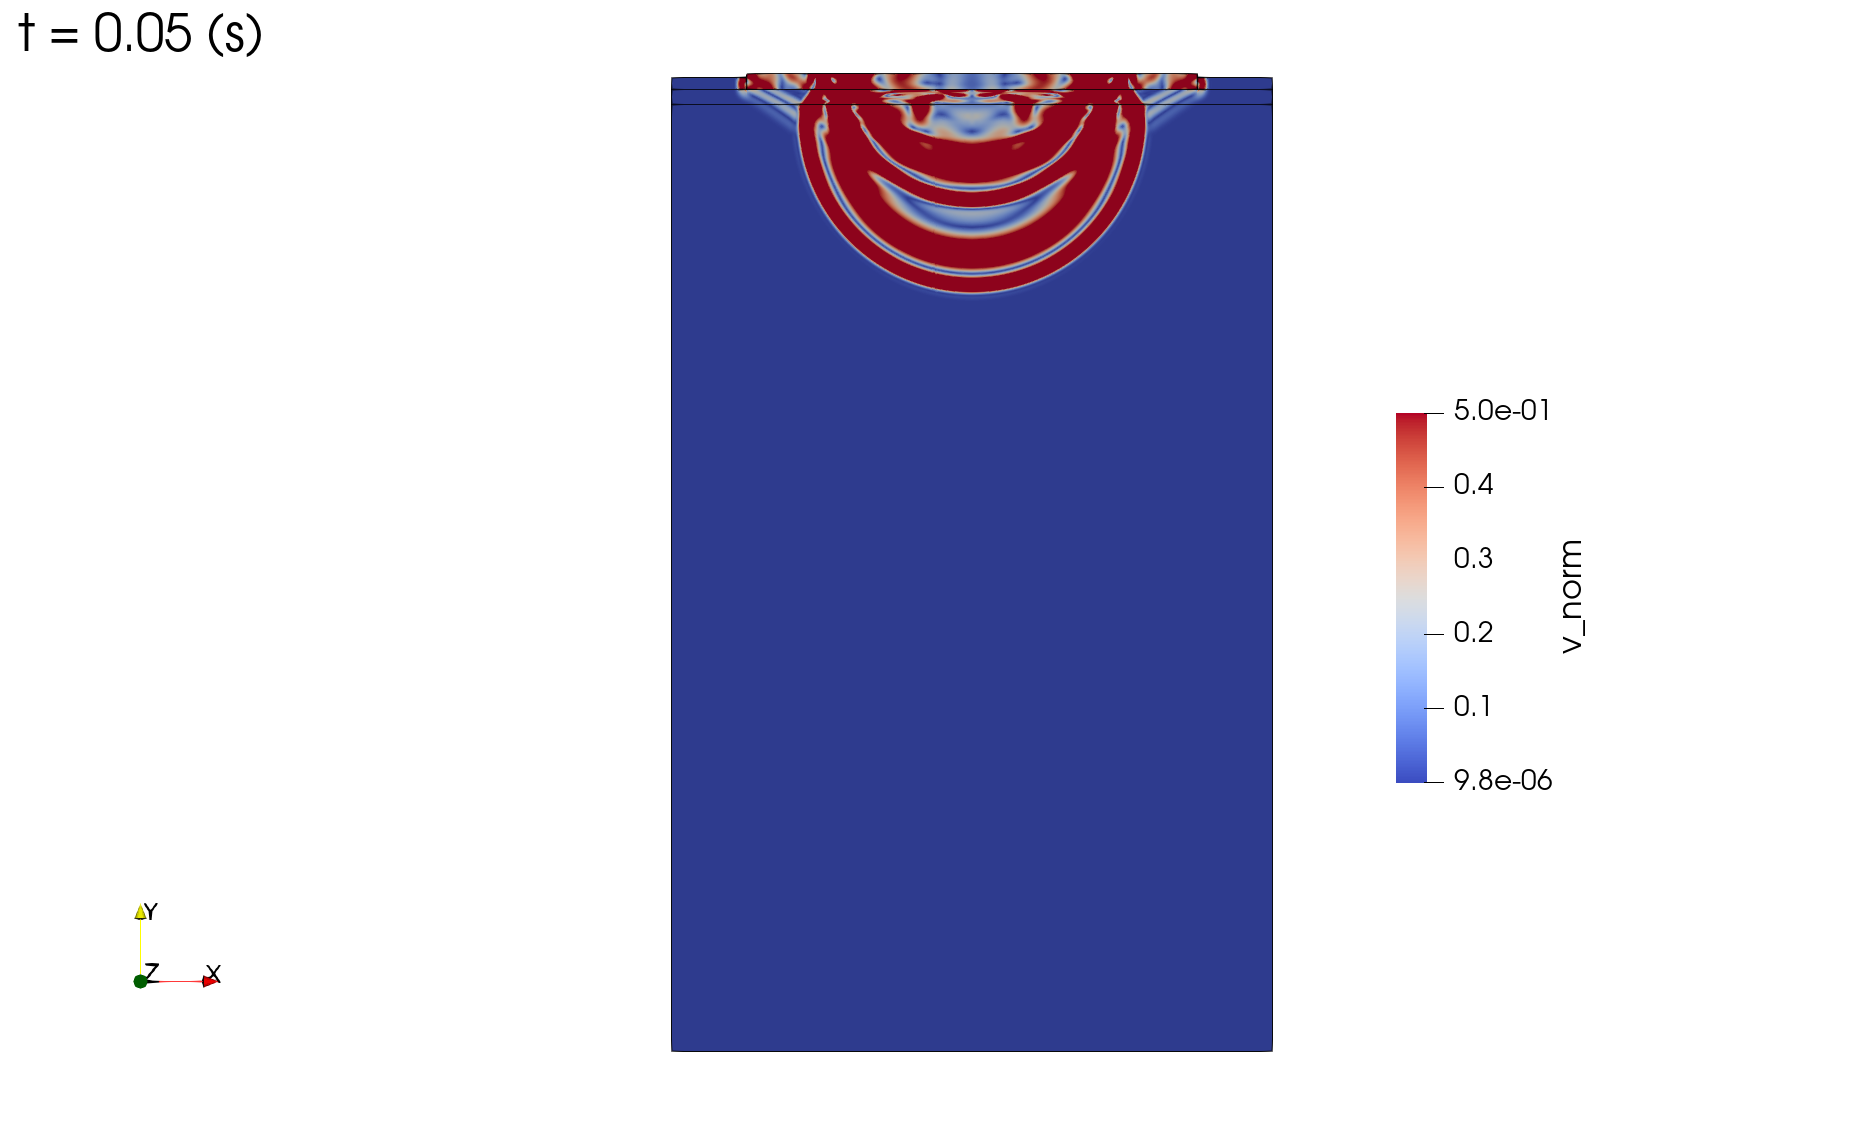
\includegraphics[trim={20cm 1cm 20cm 3cm},clip,width=0.32\textwidth]
    {images/gas_field/0.05.png}
    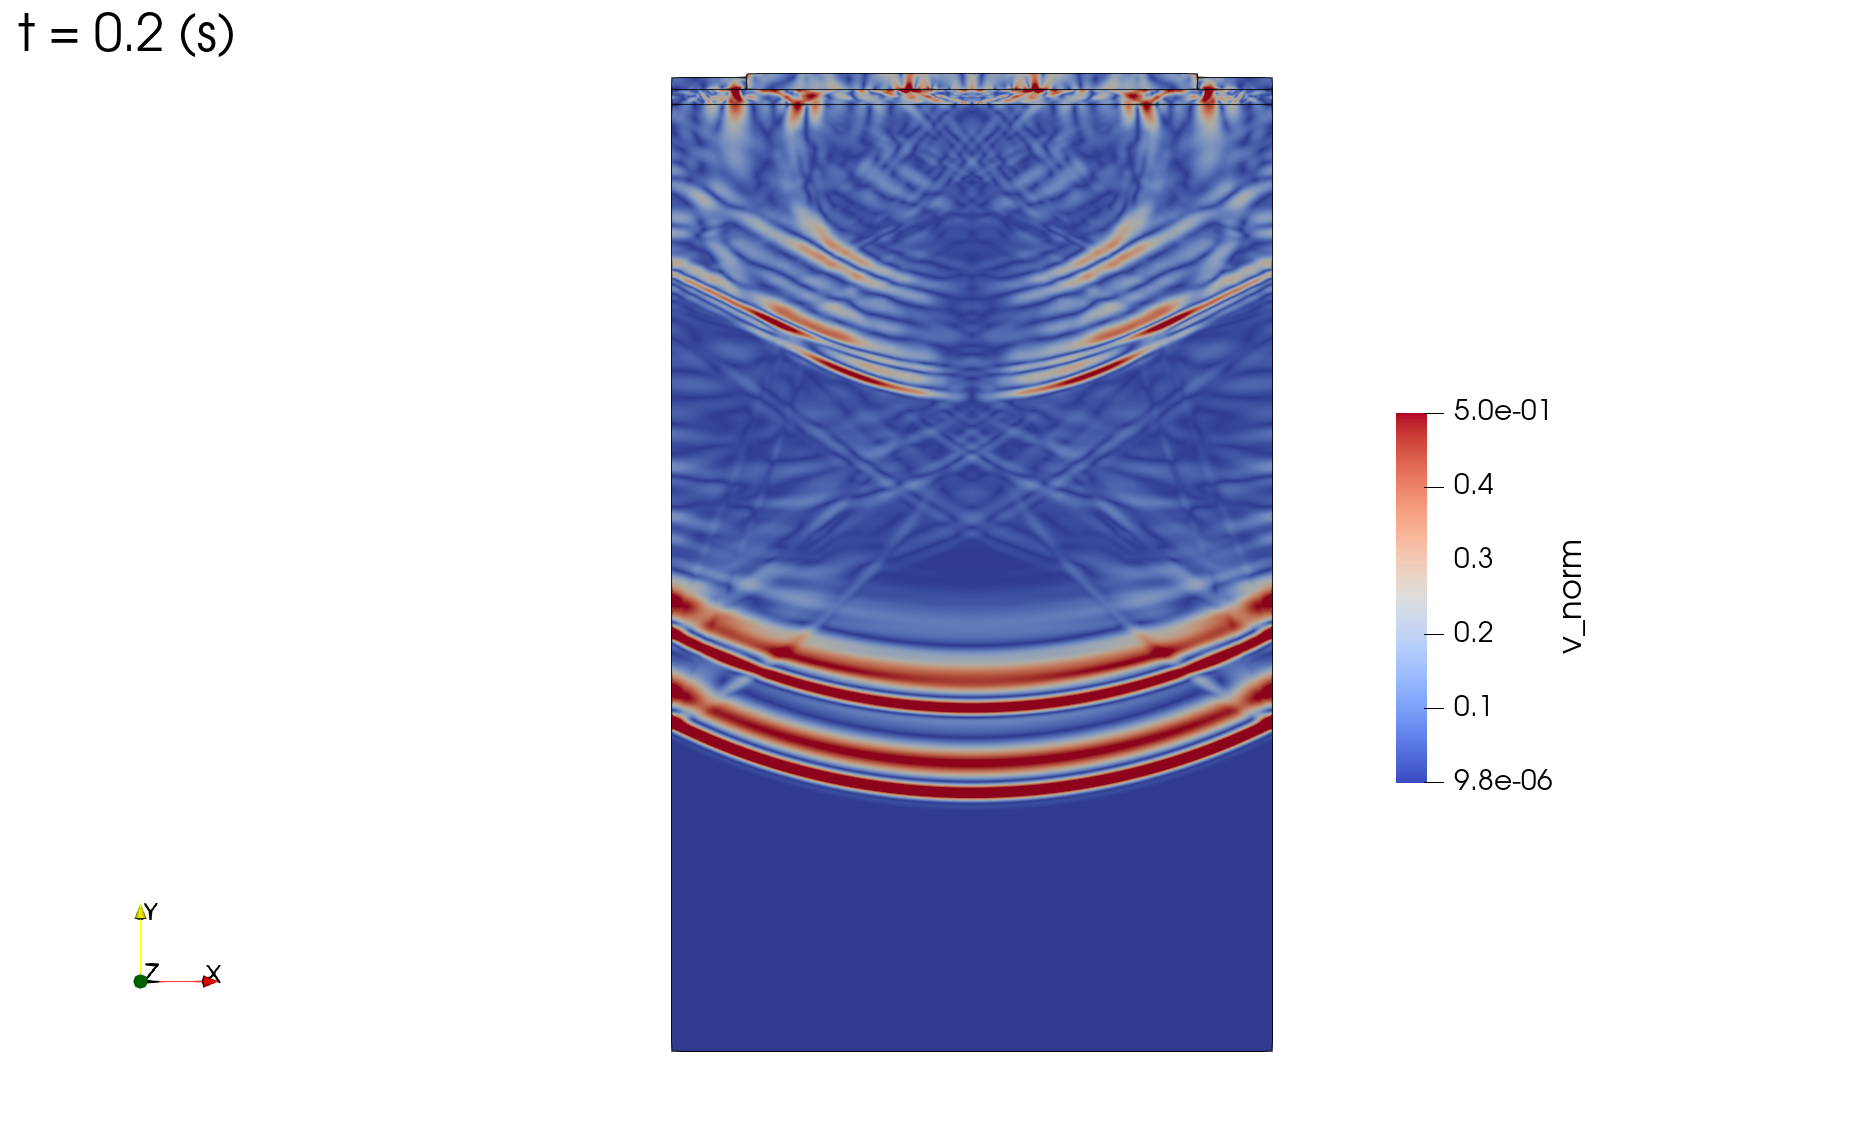
\includegraphics[trim={20cm 1cm 20cm 3cm},clip,width=0.32\textwidth]
    {images/gas_field/0.20.png}
    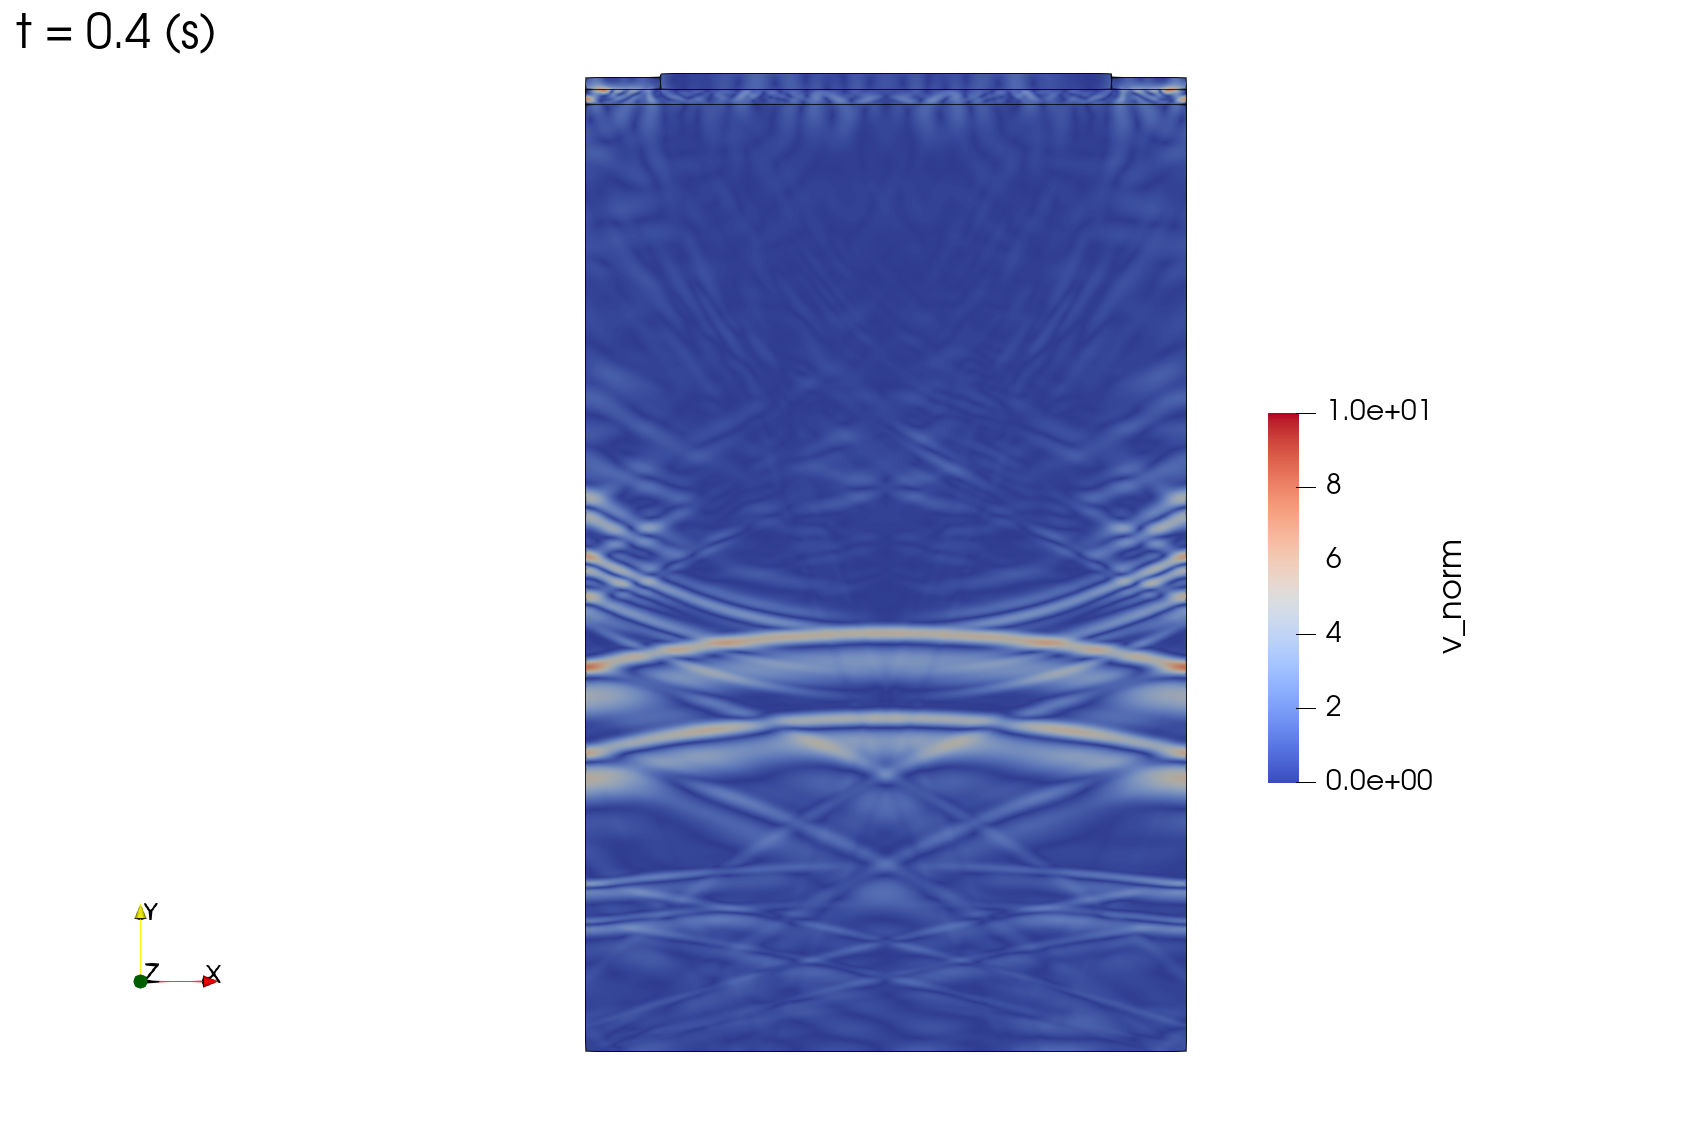
\includegraphics[trim={20cm 1cm 20cm 3cm},clip,width=0.32\textwidth]
    {images/gas_field/0.40.png}\\
    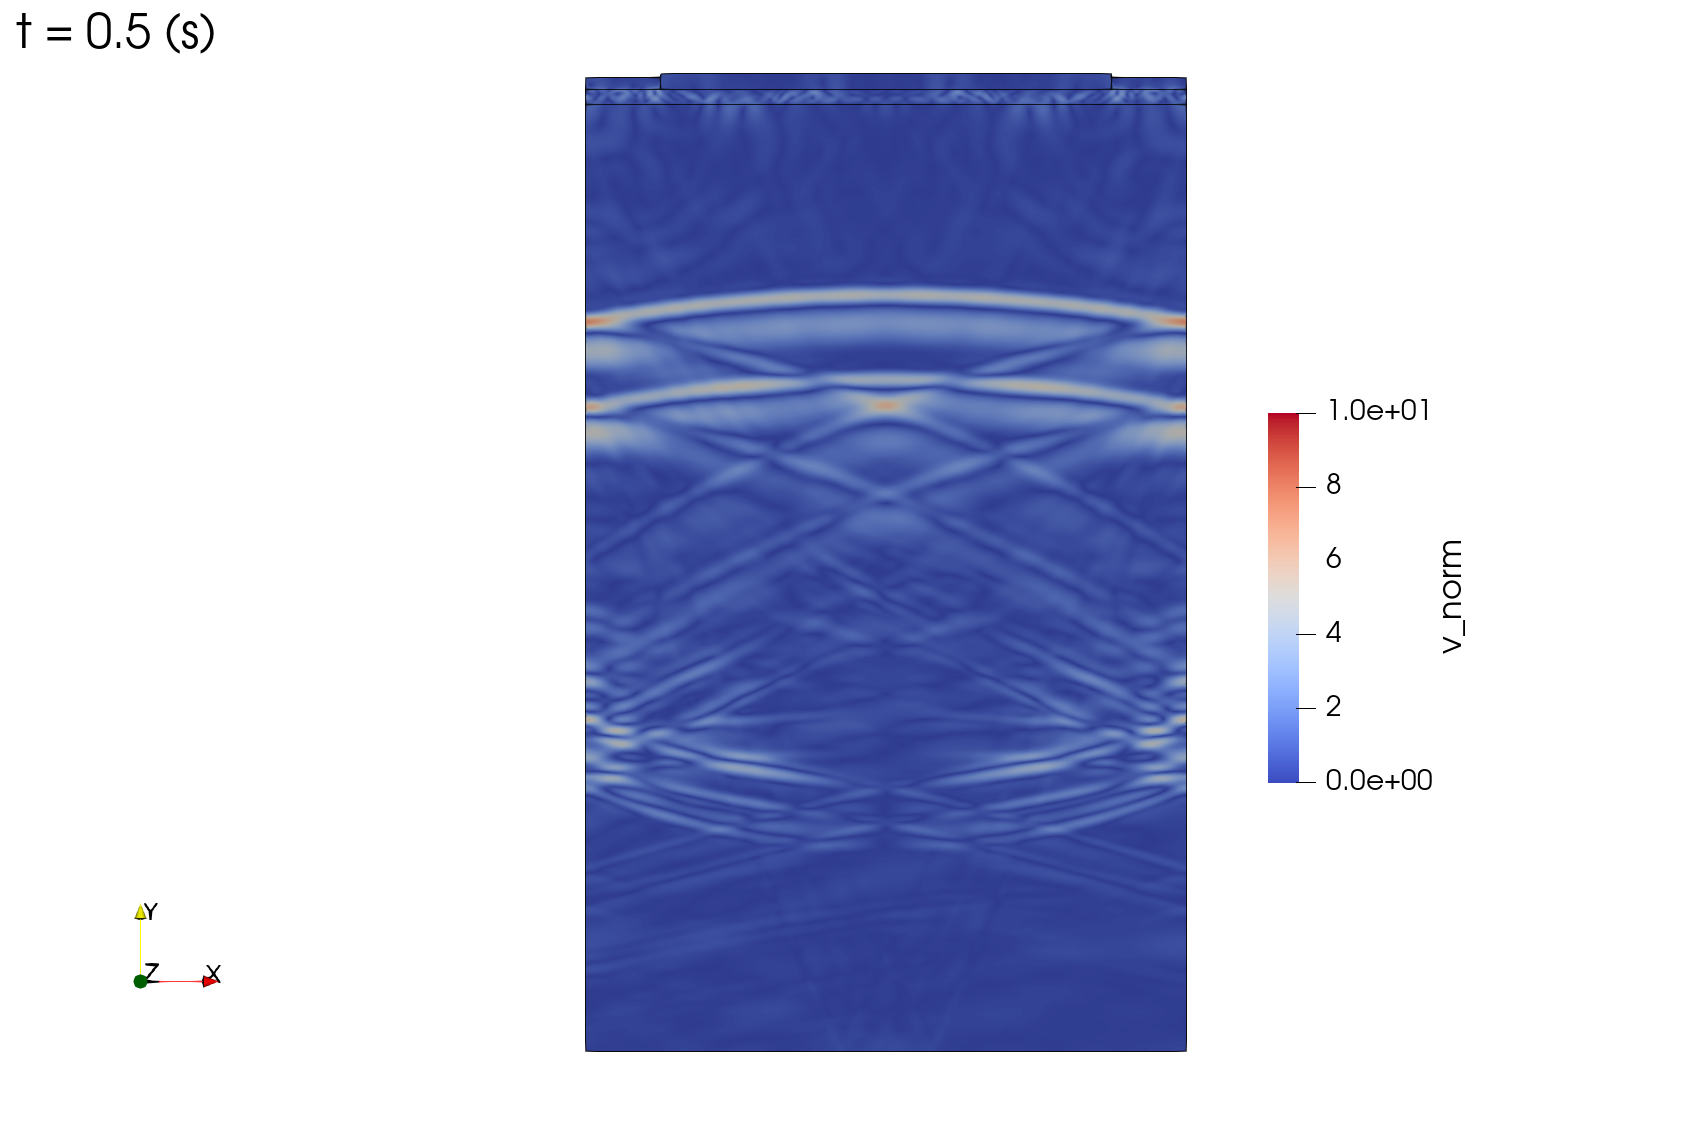
\includegraphics[trim={20cm 1cm 20cm 3cm},clip,width=0.32\textwidth]
    {images/gas_field/0.50.png}
    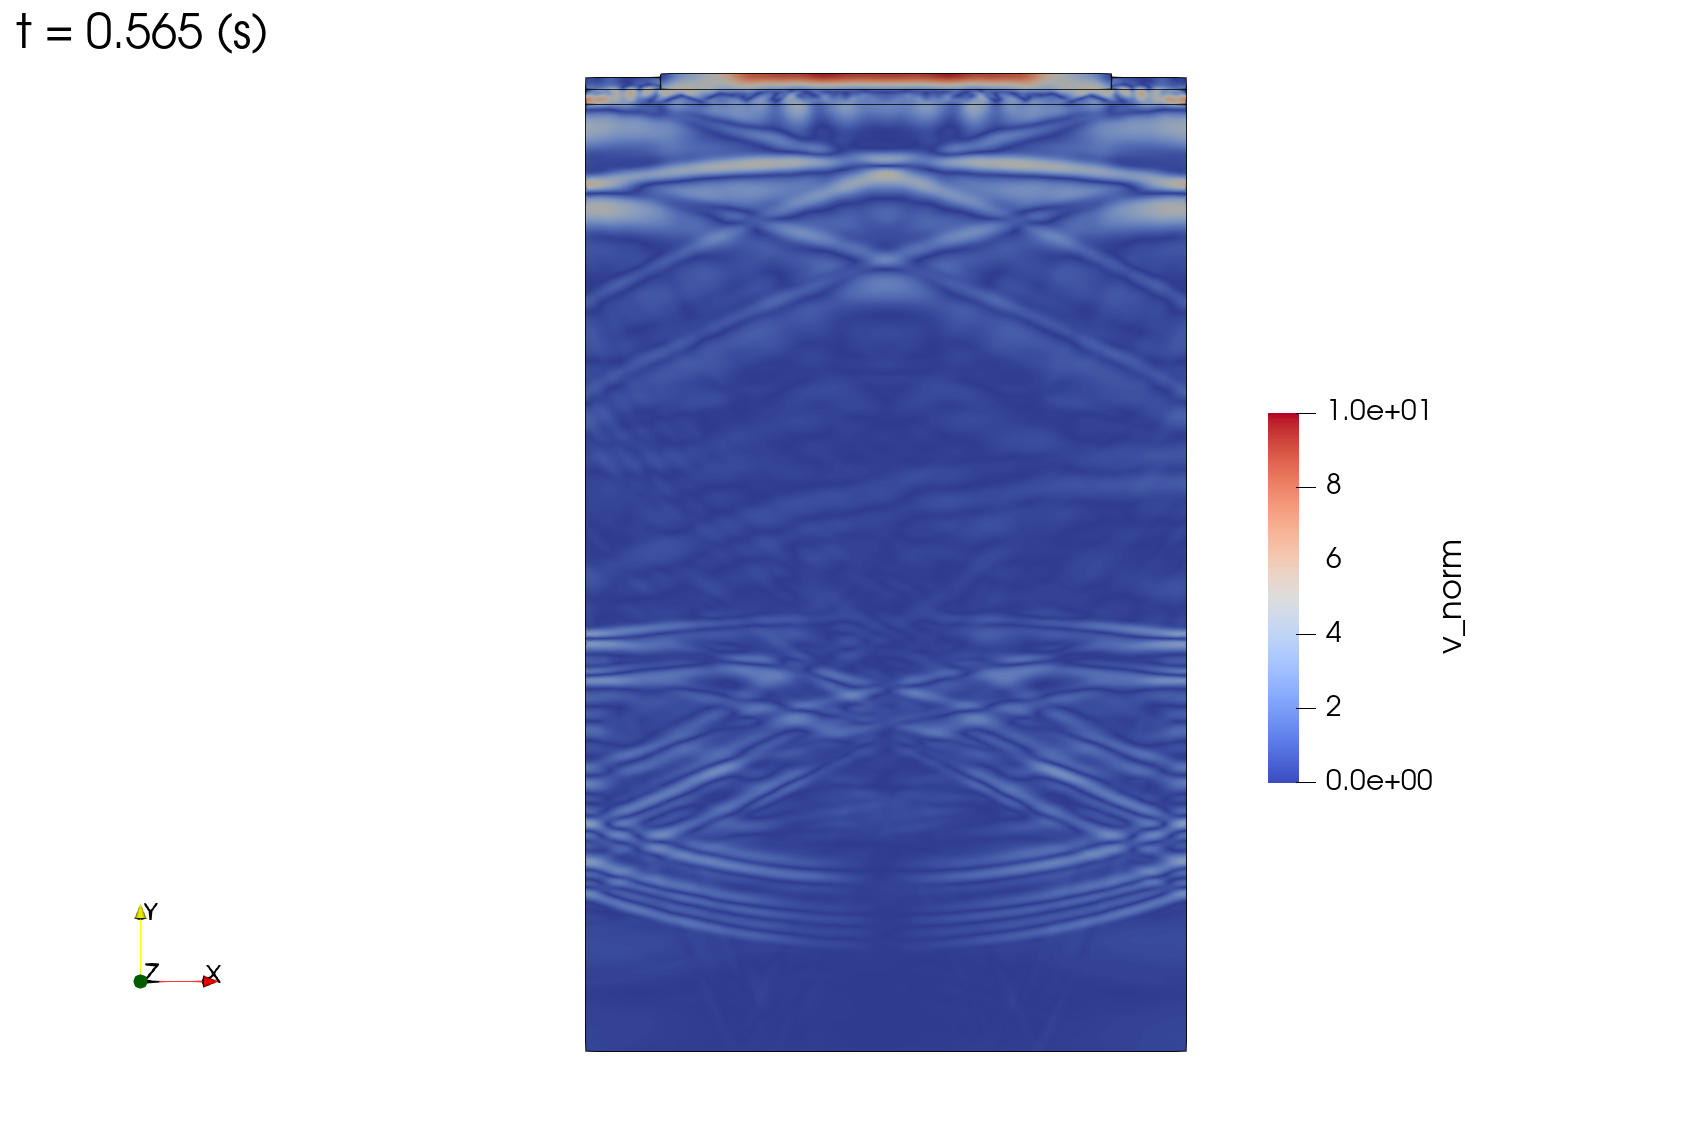
\includegraphics[trim={20cm 1cm 20cm 3cm},clip,width=0.32\textwidth]
    {images/gas_field/0.565.png}
    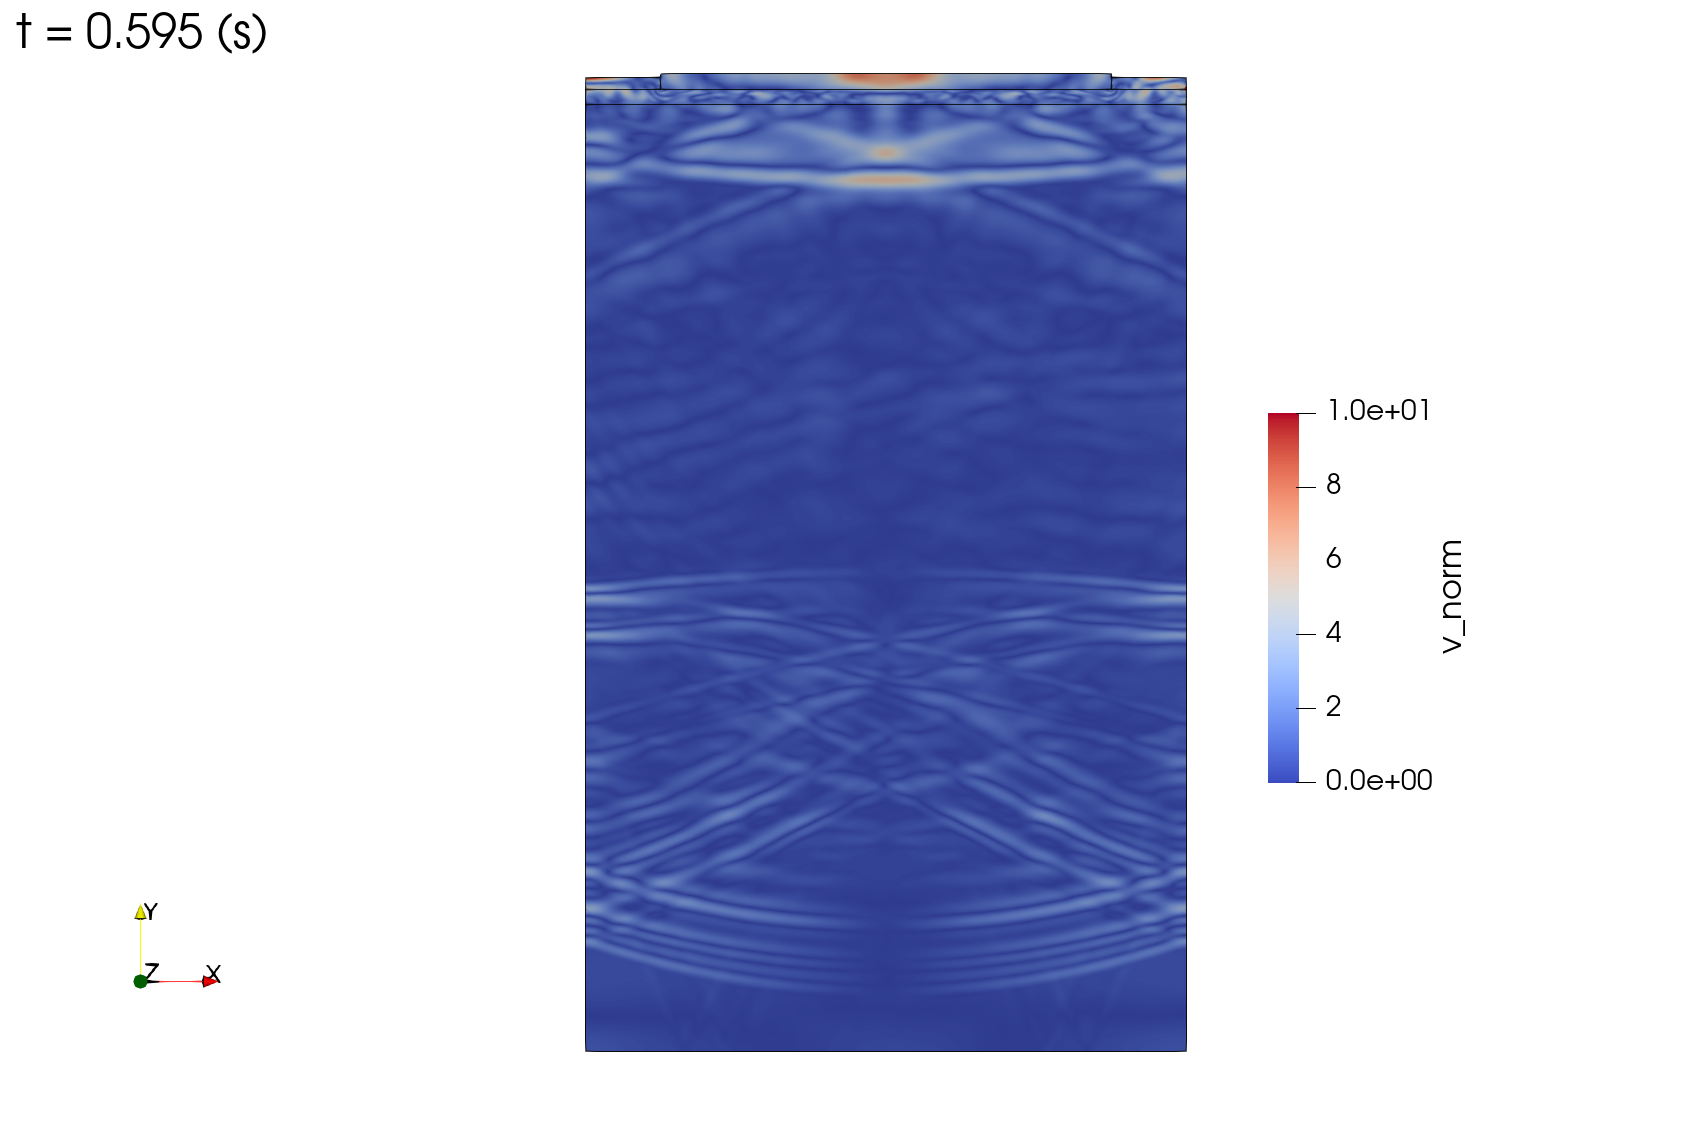
\includegraphics[trim={20cm 1cm 20cm 3cm},clip,width=0.32\textwidth]
    {images/gas_field/0.595.png}
    \caption{Волновая картина.}
    \label{fig:wave_image}
\end{figure}

\subsection{Моделирование статической нагрузки}



\section{Поглощающие граничные условия для двумерной системы уравнений акустики} \label{sec:absorbing}

При моделировании волновых процессов в геофизике зачастую приходится иметь дело с неограниченными физическими областями, в которых выделяются конечные расчётные под-области. Волны упругости, выходя за границу такой под-области, продолжают распространяться по неограниченной области, не оказывая влияния на процессы, происходящие внутри расчётной под-области. Для обеспечения такого поведения на практике,  на границах расчётных под-областей необходимо применять специальные условия.

В данной главе будут рассмотрены поглощающие граничные условия Mur и PML для систем уравнений акустики в двумерном случае.

\subsection{Уравнения акустики}


Система уравнений акустики описывает распространение малых колебаний в идеальном газе и является следствием уравнений Эйлера. В двумерном случае она имеет вид

\begin{equation}
\begin{dcases}
	\frac{\partial u}{\partial t} = -\frac{1}{\rho}\frac{\partial p}{\partial x} \\
	\frac{\partial v}{\partial t} = -\frac{1}{\rho}\frac{\partial p}{\partial y} \\
    \frac{\partial p}{\partial t} = -\rho c^2 \left(\frac{\partial u}{\partial x} + \frac{\partial v}{\partial y}\right) \\
\end{dcases}
\label{eq:acoustic}
\end{equation}

Здесь $x$ и $y$ --- координаты в ортонормированной декартовой системе координат, $u(x,y,t)$ и $v(x,y,t)$ --- скорости\footnote{Ранее в \eqref{eq:acoustic_wave_eq} мы обозначали $u\equiv v_x$, $v\equiv v_y$. Здесь переход к новым обозначениям позволяет уменьшить количество индексов, что значительно упрощает запись рассматриваемых далее численных методов.}, $p$ --- давление, $\rho$ --- плотность, $c$ --- скорость звука. Также иногда используют величину $\kappa = \rho c^2$ --- объёмный модуль упругости.

Решение системы будем рассматривать в моменты времени $t \in [0, T]$ в прямоугольной области $\Gamma := \{(x,y) ~|~ (x,y) \in [0, X]\times [0, Y]\}$.

Для краткости записи введём векторную переменную
\begin{equation}
	\varphi = \begin{pmatrix} u \\ v \\ p \end{pmatrix}
\end{equation}

Тогда начальное условие и граничные условия запишутся в следующем виде
\begin{equation}
    \varphi(x,y,0) = \varphi(x,y) ,\qquad (x,y) \in \Gamma
    \label{eq:phi}
\end{equation}
\begin{equation}
\begin{dcases}
    \varphi(0,y,t) = \varphi_L (y,t) , & y \in [0,Y]\\
    \varphi(X,y,t) = \varphi_R (y,t) , & y \in [0,Y]\\
    \varphi(x,0,t) = \varphi_T (x,t) , & x \in [0,X]\\
    \varphi(x,Y,t) = \varphi_B (x,t) , & x \in [0,X]
\end{dcases}
\end{equation}

\subsection{Численное решение системы уравнений акустики}

Здесь и далее решение дискретной задачи будем рассматривать на регулярной прямоугольной сетке с размером шага $h_x$ и $h_y$ соответственно. Для простоты будем считать, что физические размеры рассматриваемой прямоугольной области нацело делятся на шаг сетки: $X=N h_x$, $Y = M h_y$, $N,M \in \mathbb{N}$. Таким образом разностная сетка определяется как $G := \{(x_i, y_j) ~|~ x_i = ih_x, i \in \overline{0,N}, y_j = jh_y, j \in \overline{0,M} \}$. Шаг по времени будем считать постоянным равным $\tau$ и нацело делящим $T$.

При использовании значений в узлах сетки, нижние индексы будем использовать для обозначения пространственных координат, а верхний --- для времени. Например, $p_{i,j}^n$ --- давление в момент времени $t=\tau n \in [0,T]$ в точке с координатами $\left(i h_x, j h_y\right) \in G$ .

\subsubsection{Метод конечных разностей}

Простейшим численным методом решения системы уравнений в частных производных \eqref{eq:acoustic} является метод конечных разностей. Получим одну из возможных разностных схем. Для этого применим явную двухточечную схему для дискретизации производных по времени и центральную двухточечную схему для дискретизации производных по пространственным переменным.
\begin{gather*}
    \dfrac{\partial f}{\partial t} = \dfrac{f^{n+1}_{i,j} - f^{n}_{i,j}}{\tau} \\
    \dfrac{\partial f}{\partial x} = \dfrac{f^{n}_{i+1,j} - f^{n}_{i-1,j}}{2 h_x} \\
    \dfrac{\partial f}{\partial y} = \dfrac{f^{n}_{i,j+1} - f^{n}_{i,j-1}}{2 h_y}
\end{gather*}

Таким образом мы получим следующую разностную схему (leapfrog scheme)
\begin{equation}
\begin{dcases}
	\frac{u^{n+1}_{i,j} - u^{n}_{i,j}}{\tau} = -\frac{1}{\rho}\frac{p^{n+1/2}_{i+1,j} - p^{n+1/2}_{i-1,j}}{2 h_x} \\
	\frac{v^{n+1}_{i,j} - v^{n}_{i,j}}{\tau} = -\frac{1}{\rho}\frac{p^{n+1/2}_{i,j+1} - p^{n+1/2}_{i,j-1}}{2 h_y} \\
    \dfrac{p^{n+3/2}_{i,j} - p^{n+1/2}_{i,j}}{\tau}= -\rho c^2 \left(\frac{u^{n+1}_{i+1,j} - u^{n+1}_{i-1,j}}{2 h_x} + \dfrac{v^{n+1}_{i,j+1} - v^{n+1t}_{i,j-1}}{2 h_y}\right) \\
\end{dcases}
\label{eq:diff}
\end{equation}

Она имеет второй порядок аппроксимации по пространственным переменным и первый по времени.

\subsubsection{Сеточно-характеристический метод}

Более эффективным методом решения гиперболических систем является сеточно-характеристический метод. В части  \ref{sec:elastic_gcm} уже рассматривался вывод сеточно-характеристического метода для решения упругого волнового уравнения. Проведём этот вывод ещё раз, на этот раз для уравнений акустики.

Перепишем исходную систему \eqref{eq:acoustic} в матричном виде, используя раннее введённую переменную $\varphi$ \eqref{eq:phi} 
\begin{equation}
	\varphi_t = \pmb{A} \varphi_x +  \pmb{B} \varphi_y
\end{equation}

\begin{equation}
	\pmb{A} = 
	\begin{pmatrix}
		0 & 0 & -\frac{1}{\rho} \\
		0 & 0 & 0 \\
		-\rho c^2 & 0 & 0			
 	 \end{pmatrix} \qquad
	\pmb{B} = 
	\begin{pmatrix}
		0 & 0 & 0 \\
		0 & 0 & -\frac{1}{\rho} \\
		0 & -\rho c^2 & 0			
    \end{pmatrix}
\end{equation}

Для решения полученной системы воспользуемся методом расщепления: будем решать систему, делая шаг по $x$ на первом полушаге по времени, и делая шаг по $y$ на втором полушаге по времени:

\begin{equation}
\begin{gathered}
	\varphi_t = \pmb{A} \varphi_x \\
	\varphi_t = \pmb{B} \varphi_y
\end{gathered}
\label{eq:syst_split}
\end{equation} 

Таким образом пересчёт на новой временной слой будет иметь вид
\begin{equation}
\begin{gathered}
		\varphi^{t+\Delta t / 2} = S_x(\Delta t / 2, \varphi^t)\\
		\varphi^{t+\Delta t}     = S_y(\Delta t / 2, \varphi^{t+\Delta t/2})
\end{gathered}
\label{eq:gcm_t_steps}
\end{equation} 

где $\Delta t$ --- величина шага по времени, $S_x$ --- некоторый  оператор шага по $x$, $S_y$ --- шага по $y$.

Заметим, что матрицы $\pmb{A}$ и $\pmb{B}$ раскладываются как произведения

\begin{gather}
		\pmb{A} = \pmb{S}_1^{-1} \pmb{\Lambda}_1 \pmb{S}_1\\
		\pmb{B} = \pmb{S}_2^{-1} \pmb{\Lambda}_2 \pmb{S}_2
\end{gather}

где  $\pmb{\Lambda}_i$ --- диагональные матрицы, составленные из собственных чисел матриц $A$ и $B$
\begin{equation}
	\pmb{S}_1^{-1} = 
	\begin{pmatrix}
		0 & \frac{1}{\rho c} & -\frac{1}{\rho c} \\
		1 & 0 & 0 \\
		0 & 1 & 1			
    \end{pmatrix} \qquad
	\pmb{S}_1 = 
	\begin{pmatrix}
		0 & 1 & 0 \\
		\frac{\rho c}{2} & 0 & \frac{1}{2} \\
		-\frac{\rho c}{2} & 0 & \frac{1}{2}		
 	 \end{pmatrix}
\end{equation}

\begin{equation}
	\pmb{S}_2^{-1} = 
	\begin{pmatrix}
		1 & 0 & 0 \\
		0 & \frac{1}{\rho c} & -\frac{1}{\rho c} \\
		0 & 1 & 1			
 	\end{pmatrix} \qquad
	\pmb{S}_2 = 
	\begin{pmatrix}
		1 & 0 & 0 \\
		0 & \frac{\rho c}{2} & \frac{1}{2} \\
		0 & -\frac{\rho c}{2} & \frac{1}{2}	
 	\end{pmatrix}
\end{equation}

\begin{equation}
	\pmb{\Lambda}_1 = \pmb{\Lambda}_2 = 
	\begin{pmatrix}
		0 & 0 & 0 \\
		0 & -c & 0 \\
		0 & 0 & c				
	\end{pmatrix}
\end{equation}

Так как, как было показано выше, матрицы $\pmb{A}$ и $\pmb{B}$ приводятся к диагональному виду, то поставленная задача является гиперболической.

Домножим уравнения \eqref{eq:syst_split} слева на $\pmb{S}_1$ и $\pmb{S}_2$ соответственно:
\begin{equation}
\begin{gathered} 
	\pmb{S}_1\varphi_t = 
	\pmb{S}_1 \pmb{A} \varphi_x =
	\left(\pmb{S}_1 \pmb{S}_1^{-1}\right)\pmb{\Lambda}_1 \pmb{S}_1 \varphi_x =
	\pmb{\Lambda}_1 \left(\pmb{S}_1 \varphi_x \right) \\
	\pmb{S}_2\varphi_t = 
	\pmb{S}_2 \pmb{B} \varphi_y = 
	\left(\pmb{S}_2 \pmb{S}_2^{-1}\right)\pmb{\Lambda}_2 \pmb{S}_2 \varphi_y =
	\pmb{\Lambda}_2 \left(\pmb{S}_2 \varphi_y \right)
\end{gathered}
\end{equation}

Делая замену $\omega^i =  \pmb{S}_i \varphi$, $i\in\{1,2\}$, и учитывая, что матрицы $\pmb{\Lambda}_i$ диагональные, приходим к двум системам из трёх скалярных независимых уравнений переноса:

\begin{equation}
\begin{gathered} 
	\omega^1_t = \pmb{\Lambda}_1 \omega^1_x\\
	\omega^2_t = \pmb{\Lambda}_2 \omega^2_y
\end{gathered}
\end{equation}

Для решения этих скалярных уравнений будем использовать схему TVD второго порядка с ограничителем superbee.

\subsection{Виды поглощающих граничных условий}

Существует три основных подхода для реализации поглощающих граничных условий \cite{Trefethen1996FiniteDA} \cite{arch_comp_sim}:
\begin{enumerate}
    \item  Введение новых пространственных переменных, которые переводят неограниченную рассматриваемую область в ограниченную. На этот подход можно посмотреть и с <<физической>> стороны, рассматривая дискретизацию неограниченного региона сеткой с бесконечно возрастающим по мере удаления от рассматриваемой под-области шагом сетки.
    \item Анализ соотношений между падающей и отражённой волной и постановка граничного условия соответствующего минимизации отражённой части.
    \item Добавление к рассматриваемой ограниченной области новых граничных слоёв, в которых дополнительно вводится диссипативный член, растущий по мере удаления от рассматриваемой области.
\end{enumerate}

В данной работе мы будем обращаться к последним двум подходам, представленным соответственно граничными условиями Mur и PML.

\subsection{Поглощающие граничное условие Mur}

Рассмотрим одномерное волновое уравнение
\begin{equation}
    \dfrac{\partial^2 u}{\partial x^2} - \dfrac{1}{c^2}\dfrac{\partial^2 u}{\partial t^2} = 0
    \label{eq:1d_wave_eq}
\end{equation}

Это уравнение очевидно является одномерным частным случаем двумерной системы уравнений акустики \eqref{eq:acoustic} при $\varphi(x,y,t) = \varphi(x,t)$.

Разложим \eqref{eq:1d_wave_eq} на два уравнения переноса
\begin{equation}
    \dfrac{\partial u}{\partial x} - \dfrac{1}{c} \dfrac{\partial u}{\partial t} = 0
    \label{eq:left_wave}
\end{equation}
\begin{equation}
    \dfrac{\partial u}{\partial x} + \dfrac{1}{c} \dfrac{\partial u}{\partial t} = 0
    \label{eq:right_wave}
\end{equation}

Уравнение \eqref{eq:left_wave} соответствует волне, идущей влево по оси x, а уравнение \eqref{eq:right_wave} --- идущей вправо.

Пусть рассматриваемая область представляет собой отрезок $\gamma := [0, N h_x]$. Поставим поглощающее граничное условие на правом конце (для левой границы это можно сделать абсолютно аналогично). Чтобы правая граница была поглощающей, или не-отражающей, необходимо, чтобы отсутствовала отражённая волна, распространяющаяся влево. В таком случае, на правой границе должно выполняться только уравнение \eqref{eq:right_wave}, а не полное волновое уравнение \eqref{eq:1d_wave_eq}.

\begin{equation}
    \dfrac{\partial u}{\partial x} = -\dfrac{1}{c} \dfrac{\partial u}{\partial t}
\end{equation}

Для того, чтобы при дискретизации производная по времени и производная по пространственной координате были вычислены в одной точке, будем усреднять разностные производные в моменты времени $n$ и $n+1$, получая таким образом решение в точке $x = \left(N-\frac{1}{2}\right)h_x$, $t=\left(n+\frac{1}{2}\right)\tau$. \cite{arch_comp_sim}
%https://w3.pppl.gov/m3d/1dwave/ln_fdtd_1d.pdf

\begin{equation}
    \dfrac{1}{2} \left(\dfrac{u^n_N - u^n_{N-1}}{h_x} + \dfrac{u^{n+1}_N - u^n_{N-1}}{h_y} \right) = -\dfrac{1}{c} \dfrac{1}{2}\left(\dfrac{u^{n+1}_N - u^n_N}{\tau} + \dfrac{u^{n+1}_{N-1} + u^{n+1}_{N-1}}{\tau} \right)
\end{equation}

Обозначая $r = \dfrac{c \tau}{h_x}$, получаем явное выражение для граничного условия

\begin{equation}
    u^{n+1}_N = u^n_{N-1} + \dfrac{r-1}{r+1}(u^{n+1}{N-1}-u^n_N)
\end{equation}

В одномерном случае поглощающее условие Mur является точным. Распространить его можно и на двухмерный случай для рассматриваемой нами системы уравнений акустики \eqref{eq:acoustic}

\begin{equation}
    u^{n+1}_{N,j} = u^n_{N-1,j} + \dfrac{r-1}{r+1}(u^{n+1}{N-1,j}-u^n_{N,j})
\end{equation}

В этом случае поглощение будет точным только если волна падает строго нормально на рассматриваемую границу, соответствуя тем самым одномерному случаю. В противном случае будет наблюдаться  возникновение отражённых от границы волн.

\subsection{Berenger PML}

Поглощающее граничное условие \textit{perfectly matched layer} (PML) впервые было введено в работе \cite{berenger} для системы уравнений Максвелла, описывающих распространение электромагнитных волн. Оказывается \cite{pml_from_maxwell}, что, произведя необходимые замены переменных, эту систему уравнений можно свести к системе уравнений акустики \eqref{eq:acoustic}.

Для реализации затухания в PML слое добавляются диссипативные слагаемые $c u \sigma_x(x,y)$ и $c u \sigma_y(x,y)$, где в качестве функций $\sigma_{x/y}$ обычно выбирают

\begin{equation}
\begin{gathered}
	\sigma_x = \left(\frac{d_x}{w_{x}}\right)^k \Sigma_{x}\\
	\sigma_y = \left(\frac{d_y}{w_{y}}\right)^k \Sigma_{y}
\end{gathered}
\label{eq:pml_coefs}
\end{equation}

здесь $d_{x/y}(x,y)$ --- глубина проникновения в PML слой, имеющий глубину $w_{x/y}$, $k$ --- степень скорости роста коэффициентов PML, $\Sigma_{x/y}$ --- максимальные значения диссипативных слагаемых\footnote{Глубина проникновения в PML слой очевидно меньше ширины слоя, а значит множитель перед $\Sigma_{x/y}$ лежит в пределах от 0 до 1. Значит $\sigma_{x/y}$ лежит в пределах от 0 до $\Sigma_{x/y}$.}. 

\begin{figure}[htp]
    \centering
    \includegraphics[trim={72pt 325pt 430pt 55pt},clip,width=0.4\textwidth]{images/pml/pml_scheme.png}
    \caption{Схема правого и верхнего PML слоёв.}
    \label{fig:pml_scheme}
\end{figure}

Значения параметров $k$ и $\Sigma_{x,y}$ обычно подбираются под конкретную задачу из эмпирических соображений для наиболее эффективной реализации поглощающего граничного условия.

В случае применения PML на всех четырёх границах прямоугольной области $\Gamma$, то, используя обозначения, введённые для рассчётной сетки $G$, можно записать
    
\begin{gather}
	d_x = h_x \cdot \min\{i, N - i\} \\
	d_y = h_y \cdot \min\{j, M - j\}  
\end{gather}
    
Система уравнений акустики c диссипативными членами имеет вид \cite{pml_from_maxwell}
    
\begin{equation}
	\begin{dcases}
		\frac{\partial u}{\partial t} + c\sigma_x u = -\frac{1}{\rho}\frac{\partial p}{\partial x} \\
		\frac{\partial v}{\partial t} + c\sigma_y u = -\frac{1}{\rho}\frac{\partial p}{\partial y} \\
	    \frac{\partial p}{\partial t} + c(\sigma_x + \sigma_y) p = -\rho c^2 \left(\frac{\partial u}{\partial x}+\frac{\partial v}{\partial y}\right) - \rho c^2 \sigma_x \frac{\partial Q}{\partial y} - \rho c^2 \sigma_y \frac{\partial P}{\partial x} \\
	    \frac{\partial Q}{\partial t} = cv \\
	    \frac{\partial P}{\partial t} = cu
	\end{dcases}\label{eq:pml} 
\end{equation}
    
где $Q$ и $P$ --- дополнительные переменные, определяющиеся из последних двух уравнений.
    
\subsection{Split-field PML}

Другим классическим вариантом граничного условия PML является так называемый \textit{split-field PML} \cite{aaaaaaaaaa}

\begin{equation}
	\begin{dcases}
	    \left(\frac{\partial}{\partial t} + \sigma_x(x)\right) p_1 + \kappa \frac{\partial}{\partial x} v_x = 0 \\
	    \left(\frac{\partial}{\partial t} + \sigma_y(y)\right) p_2 + \kappa \frac{\partial}{\partial y} v_y = 0 \\
	    \left(\frac{\partial}{\partial t} + \sigma_x(x)\right) v_x + \frac{1}{\rho} \frac{\partial}{\partial x} p = 0 \\
	    \left(\frac{\partial}{\partial t} + \sigma_y(y)\right) v_y + \frac{1}{\rho} \frac{\partial}{\partial y} p = 0 \\
	    p = p_1 + p_2
	\end{dcases}\label{eq:split_pml} 
\end{equation}
    
где, напомним,  $\kappa = \rho c^2$ --- объёмный модуль упругости. Функции $\sigma_{x/y}$ выбираются аналогично случаю Berenger PML.

В системе \eqref{eq:split_pml} давление $p$ разделяется на  компоненты $p_1$ и $p_2$. В начальный момент времени они определяются как половины общего значения давления $p$: $p_1(x,y,t=0) = p_2(x,y,t=0) = \frac{p(x,y)}{2}$. В дальнейшем $p_1$ и $p_1$ определяются из численных уравнений, а $p$ вычисляется после каждой итерации, как сумма $p_1$ и $p_2$. 
    
\subsection{Решение PML-систем методом конечных разностей}
    
Аналогично разностной схеме \eqref{eq:diff} для системы уравнений  акустики, заменяя аналитические производные на разностные, получим системы разностных уравнений для Berenger PML \eqref{eq:pml}
    
\begin{equation}
	\begin{dcases}
		\frac{u^{n+1}_{i,j} - u^{n}_{i,j}}{\tau} + c \sigma_{x_{i}} u^{n} = -\frac{1}{\rho}\frac{p^{n+\sfrac{1}{2}}_{i+\sfrac{1}{2},j} - p^{n+\sfrac{1}{2}}_{i-\sfrac{1}{2},j}}{h_x} \\
		\frac{v^{n+1}_{i,j} - v^{n}_{i,j}}{\tau} + c \sigma_{y_{j}} v^{n}  = -\frac{1}{\rho}\frac{p^{n+\sfrac{1}{2}}_{i,j+1} - p^{n+\sfrac{1}{2}}_{i,j-1}}{2h_y} \\
		\frac{Q^{n+1} - Q^{n}}{\tau} = c v^n_{i,j}\\
		\frac{P^{n+1} - P^{n}}{\tau} = c u^n_{i,j}\\
	    \dfrac{p^{n+\sfrac{3}{2}}_{i,j} - p^{n+\sfrac{1}{2}}_{i,j}}{\tau} + c \left(\sigma_{x_{i}} + \sigma_{y_{j}}\right)p^{n+\sfrac{1}{2}} =\\= -\rho c^2 \left(\frac{u^{n+1}_{i+1,j} - u^{n+1}_{i-1,j}}{2h_x} + \dfrac{v^{n+1}_{i,j+1} - v^{n+1}_{i,j-1}}{2h_y} - \sigma_{x_i}\frac{Q^{n+1}_{i,j+1} - Q^{n+1}_{i,j}}{h_y} - \sigma_{y_j}\frac{P^{n+1}_{i+1,j} - P^{n+1}_{i,j}}{h_x} \right)
	\end{dcases}\label{eq:diff_pml}
\end{equation}
    
и для split-field PML \eqref{eq:split_pml}
\begin{equation}
    \begin{dcases}
        (p_1)_{i,j}^{n+1}
        p_{i,j}^{n+1} = (p_1)_{i,j}^{n+1} + (p_2)_{i,j}^{n+1}
    \end{dcases}
    \label{eq:diff_split_pml}
\end{equation}
    
\subsection{Решение PML-систем сеточно-характеристическим методом}
    
Cеточно-характеристический метод, рассмотренный в первой главе, является более эффективным по сравнению с простым конечно-разностным методом. Покажем, что он применим для решения систем уравнений Berenger PML \eqref{eq:pml} и split-field pml \eqref{eq:split_pml}.
    
\subsubsection{Berenger PML}
    
Рассмотрим систему уравнений, реализующую затухающее граничнее условие типа PML \eqref{eq:pml}, и произведём замену:
\begin{equation}
    \varphi = \begin{pmatrix}
        u \\ v \\ p \\ Q \\ P
    \end{pmatrix}
\end{equation}
    
Тогда система принимает вид
\begin{equation}
    \varphi_t = \pmb{A}\varphi_x + \pmb{B}\varphi_y + \pmb{S}\varphi
\end{equation}

где матрицы $\pmb{A}$, $\pmb{B}$ и $\pmb{S}$ следующие
\begin{equation*}
    \pmb{A} = \begin{pmatrix}
        0 & 0 & -\frac{1}{\rho} & 0 & 0 \\
        0 & 0 & 0 & 0 & 0 \\
        -\rho c^2 & 0 & 0 & 0 & -\rho c^2 \sigma_y \\
        0 & 0 & 0 & 0 & 0 \\
        0 & 0 & 0 & 0 & 0
    \end{pmatrix} \qquad
	\pmb{B} = \begin{pmatrix}
        0 & 0 & 0 & 0 & 0 \\
        0 & 0 & -\frac{1}{\rho} & 0 & 0 \\
        0 & -\rho c^2  & 0 & -\rho c^2 \sigma_x & 0 \\
        0 & 0 & 0 & 0 & 0 \\
        0 & 0 & 0 & 0 & 0
    \end{pmatrix}
\end{equation*}
    
\begin{equation*}
	\pmb{S} = \begin{pmatrix}
        -c \sigma_x & 0 & 0 & 0 & 0 \\
        0 & -c \sigma_y & 0 & 0 & 0 \\
        0 & 0 & -c (\sigma_x + \sigma_y) & 0 & 0 \\
        0 & c & 0 & 0 & 0 \\
        c & 0 & 0 & 0 & 0
    \end{pmatrix}
\end{equation*}

Эти матрицы можно диагонализовать

\begin{equation*}
    \pmb{A} = \pmb{L}_1 \pmb{\Lambda}_1 \pmb{R}_1
\end{equation*}
\begin{equation*}
    \pmb{B} = \pmb{L}_2 \pmb{\Lambda}_2 \pmb{R}_2
\end{equation*}
\begin{equation*}
    \pmb{S} =\pmb{L}_3 \pmb{\Lambda}_3 \pmb{R}_3
\end{equation*}


\begin{equation*}
    \pmb{L}_1 = \begin{pmatrix}
        0 & 0 & 1 & 0 & 0 \\
        0 & -\sigma_y & 0 & \frac{1}{c \rho} & -\frac{1}{c \rho} \\
        0 & 0 & 0 & 1 & 1 \\
        0 & 1 & 0 & 0 & 0 \\
        1 & 0 & 0 & 0 & 0
    \end{pmatrix} \qquad
    \pmb{R}_1 = \begin{pmatrix}
        0 & 0 & 0 & 0 & 1 \\
        0 & 0 & 0 & 1 & 0 \\
        1 & 0 & 0 & 0 & 0 \\
        0 & \frac{c \rho}{2} & \frac{1}{2} & \frac{c \rho \sigma_y}{2} & 0  \\
        0 & -\frac{c \rho}{2}  & \frac{1}{2} & - \frac{c \rho \sigma_y}{2} & 0
    \end{pmatrix}
\end{equation*}
    
\begin{equation*}
    \pmb{L}_2 = \begin{pmatrix}
        -\sigma_x & 0 & 0 & \frac{1}{c \rho} & -\frac{1}{c \rho} \\
        0 & 0 & 1 & 0 & 0 \\
        0 & 0 & 0 & 1 & 1 \\
        0 & 1 & 0 & 0 & 0 \\
        1 & 0 & 0 & 0 & 0
    \end{pmatrix} \qquad
    \pmb{R}_2 = \begin{pmatrix}
        0 & 0 & 0 & 0 & 1 \\
        0 & 0 & 0 & 1 & 0 \\
        0 & 1 & 0 & 0 & 0 \\
        \frac{c \rho}{2} & 0 & \frac{1}{2} & 0 & \frac{c \rho \sigma_x}{2}  \\
        -\frac{c \rho}{2} & 0 & \frac{1}{2} & 0 & - \frac{c \rho \sigma_x}{2} 
    \end{pmatrix}
\end{equation*}

\begin{equation*}
    \pmb{\Lambda}_1 = \pmb{\Lambda}_2 = \begin{pmatrix}
        0 & 0 & 0 & 0 & 0 \\
        0 & 0 & 0 & 0 & 0 \\
        0 & 0 & 0 & 0 & 0 \\
        0 & 0 & 0 & -c & 0 \\
        0 & 0 & 0 & 0 & c
    \end{pmatrix} 
\end{equation*}
    

\begin{equation*}
    \pmb{L}_3 = \begin{pmatrix}
        0 & 0 & -\sigma_x & 0 & 0 \\
        0 & 0 & 0 & -\sigma_y & 0 \\
        0 & 0 & 0 & 0 & 1 \\
        0 & 1 & 0 & 1 & 0 \\
        1 & 0 & 1 & 0 & 0
    \end{pmatrix} \qquad
    \pmb{R}_3 = \begin{pmatrix}
        \sigma_x^{-1} & 0 & 0 & 0 & 1 \\
        0 & \sigma_y^{-1} & 0 & 1 & 0 \\
        -\sigma_x^{-1} & 0 & 0 & 0 & 0 \\
        0 & -\sigma_y^{-1} & 0 & 0 & 0 \\
        0 & 0 & 1 & 0 & 0
    \end{pmatrix}
\end{equation*}

\begin{equation*}
    \pmb{\Lambda}_3 = \begin{pmatrix}
        0 & 0 & 0 & 0 & 0 \\
        0 & 0 & 0 & 0 & 0 \\
        0 & 0 & -c \sigma_x & 0 & 0 \\
        0 & 0 & 0 & -c \sigma_y & 0 \\
        0 & 0 & 0 & 0 & -c (\sigma_x + \sigma_y)
    \end{pmatrix}
\end{equation*}

Полученное векторное уравнение в частных производных можно расщепить по физическим процессам для каждой компоненты аналогично уравнению переноса-диффузии с $\mu = 0$ \cite{rashep_marchuk}.

Будем решать систему, делая шаг по $x$ на первой трети шага по времени, делая шаг по $y$ на второй, и решая неоднородное уравнение на третей части шага по времени:
\begin{gather*} 
	\label{eq:pml_eq_split_1} \varphi_t = \pmb{A} \varphi_x \\
	\label{eq:pml_eq_split_2} \varphi_t = \pmb{B} \varphi_y \\
	\label{eq:pml_eq_split_3} \varphi_t = \pmb{S} \varphi
\end{gather*}

Домножая $i$-ое уравнение слева на $\pmb{R_i}$
\begin{gather*} 
    \pmb{R}_1 \varphi_t = \pmb{R}_1\left(\pmb{L}_1 \pmb{\Lambda}_1 \pmb{R}_1\right) \varphi_x \\
	\pmb{R}_2 \varphi_t = \pmb{R}_2\left(\pmb{L}_2 \pmb{\Lambda}_2 \pmb{R}_2\right) \varphi_y \\
	\pmb{R}_3 \varphi_t = \pmb{R}_3\left(\pmb{L}_3 \pmb{\Lambda}_3\pmb{ R}_3\right) \varphi
\end{gather*}
\begin{gather*} 
    \pmb{R}_1 \varphi_t = \pmb{\Lambda}_1 \pmb{R}_1 \varphi_x \\
	\pmb{R}_2 \varphi_t = \pmb{\Lambda}_2 \pmb{R}_2 \varphi_y \\
	\pmb{R}_3 \varphi_t = \pmb{\Lambda}_3 \pmb{R}_3 \varphi
\end{gather*}
    
Делая замену $\omega^i = \pmb{R}_i\varphi $, $i\in\{1,2,3\}$, и учитывая, что матрицы $\pmb{\Lambda}_i$ диагональные, приходим к трём системам из трёх скалярных независимых уравнений:
\begin{equation}
\begin{dcases}
    \omega^1_t = \pmb{\Lambda}_1 \omega^1_x \\
	\omega^2_t = \pmb{\Lambda}_2 \omega^2_y \\
	\omega^3_t = \pmb{\Lambda}_3 \omega^3
\end{dcases}
\label{eq:pml_grid_char_sys}
\end{equation}

Первые две системы представляют собой независимые скалярные уравнения переноса. Для их численного решения мы  воспользуемся TVD-схемой второго порядка с ограничителем superbee.
    
Третья система представляет собой 5 независимых скалярных уравнений с разделяемыми переменными, которые очевидно решаются аналитически. Обозначая номер уравнения нижним индексом $l$, получаем

\begin{equation*}
\begin{dcases}
    \left(\omega^3_l\right)_t = 0 & l=1,2\\
    \left(\omega^3_l\right)_t = \left[\pmb{\Lambda}_3\right]_{ll} \omega^3_l & l=3,4,5
\end{dcases}
\end{equation*}

\begin{equation*}
\begin{dcases}
    \omega^3_l(t) = \omega^3_l(t=0) & l=1,2 \\
    \omega^3_l(t) = \omega^3_l(t=0) \cdot \exp\left(\left[\pmb{\Lambda}_3\right]_{ll} t\right) & l = 3,4,5
\end{dcases}
\end{equation*}

Таким образом построен сеточно-характеристический метод решения уравнения \eqref{eq:pml}.

\subsubsection{Split-Field PML}

Теперь построим сеточно-характеристический метод решения системы уравнений split-field PML \eqref{eq:split_pml}

На этот раз произведём замену
\begin{equation}
	\varphi = \begin{pmatrix} u \\ v \\ p_1 \\ p_2 \end{pmatrix}
\end{equation}

Тогда система принимает вид
\begin{equation}
	\varphi_t = \pmb{A} \varphi_x +  \pmb{B} \varphi_y - \pmb{C} \varphi
\end{equation}
где 
\begin{equation}
	\pmb{A} = 
	\begin{pmatrix}
    	0 & 0 & \frac{1}{\rho} & \frac{1}{\rho} \\
    	0 & 0 & 0 & 0 \\
        \kappa & 0 & 0 & 0 \\
    	0 & 0 & 0 & 0
	\end{pmatrix} \qquad
	\pmb{B} = 
	\begin{pmatrix}
    	0 & 0 & 0 & 0 \\
        0 & 0 & \frac{1}{\rho} & \frac{1}{\rho} \\
    	0 & 0 & 0 & 0 \\
        0 & \kappa  & 0 & 0
	\end{pmatrix} \qquad
	\pmb{C} = 
	\begin{pmatrix}
    	\sigma_x & 0 & 0 & 0 \\
    	0 & \sigma_y & 0 & 0 \\
        0 & 0 & \sigma_x & 0 \\
    	0 & 0 & 0 & \sigma_y
	\end{pmatrix}
\end{equation}

Опять замечаем, что матрицы можно диагонализовать
\begin{gather*}
	\pmb{A} = \pmb{L}_1 \pmb{\Lambda}_1 \pmb{R}_1 = 
	\begin{pmatrix}
    	0 & 0 & -\frac{1}{\sqrt{\kappa\rho}} & \frac{1}{\sqrt{\kappa\rho}} \\
    	0 & 1 & 0 & 0 \\
        -1 & 0 & 1 & 1 \\
    	1 & 0 & 0 & 0
	\end{pmatrix} 
	\begin{pmatrix}
    	0 & 0 & 0 & 0 \\
    	0 & 0 & 0 & 0 \\
        0 & 0 & -\sqrt{\frac{\kappa}{\rho}} & 0 \\
    	0 & 0 & 0 & \sqrt{\frac{\kappa}{\rho}}
	\end{pmatrix} 
	\begin{pmatrix}
    	0 & 0 & 0 & 1 \\
    	0 & 1 & 0 & 0 \\
        -\frac{\sqrt{\kappa\rho}}{2} & 0 & \frac{1}{2} & \frac{1}{2} \\
        \frac{\sqrt{\kappa\rho}}{2} & 0 & \frac{1}{2} & \frac{1}{2}
	\end{pmatrix} \\
	\pmb{B} = \pmb{L}_2 \pmb{\Lambda}_2 \pmb{R}_2 = 
	\begin{pmatrix}
    	0 & 1 & 0 & 0 \\
    	0 & 0 & -\frac{1}{\sqrt{\kappa\rho}} & \frac{1}{\sqrt{\kappa\rho}} \\
    	-1 & 0 & 0 & 0 \\
        1 & 0 & 1 & 1 
	\end{pmatrix} 
	\begin{pmatrix}
    	0 & 0 & 0 & 0 \\
    	0 & 0 & 0 & 0 \\
        0 & 0 & -\sqrt{\frac{\kappa}{\rho}} & 0 \\
    	0 & 0 & 0 & \sqrt{\frac{\kappa}{\rho}}
	\end{pmatrix} 
	\begin{pmatrix}
    	0 & 0 & -1 & 0 \\
    	1 & 0 & 0 & 0 \\
        0 & -\frac{\sqrt{\kappa\rho}}{2} & \frac{1}{2} & \frac{1}{2} \\
        0 & \frac{\sqrt{\kappa\rho}}{2}  & \frac{1}{2} & \frac{1}{2}
	\end{pmatrix} 
\end{gather*}

Опять воспользуемся расщеплением по физическим процессам для каждой компоненты полученного векторного уравнение в частных \cite{rashep_marchuk}. Тогда, расщепляя систему и домножая на $\pmb{L_i}^{-1}=\pmb{R_i}$ слева, получим
\begin{equation}
    \begin{dcases}
        \pmb{R}_1\varphi_t = \pmb{\Lambda}_1\pmb{R}_1 \varphi_x\\
        \pmb{R}_2\varphi_t = \pmb{\Lambda}_2\pmb{R}_2 \varphi_y\\
        \varphi_t = - \pmb{C} \varphi  
    \end{dcases}
\end{equation}

Производя замену переменныx $\omega_i = \pmb{R}_i \varphi$:
\begin{equation}
    \begin{dcases}
        \omega_t^1 = \pmb{\Lambda}_1\omega_x^1 \\
        \omega_t^2 = \pmb{\Lambda}_2\omega_y^2 \\
        \varphi_t = - \pmb{C} \varphi  
    \end{dcases}
\end{equation}

Решение этой системы аналогично уже разобранному решению системы \eqref{eq:pml_grid_char_sys}. 

Таким образом система уравнений split-field PML \eqref{eq:split_pml} также решается сеточно-характеристическим методом.

\subsection{Численные эксперименты}

Сравним эффективность описанных в предыдущей части поглощающих граничных условий: Mur, конечно-разностной реализации Berenger PML, сеточно-характеристической реализации Berenger PML, конечно-разностной реализация split-field PML, и, наконец, сеточно-характеристической реализации split-field PML.

\subsubsection{Область моделирования}

Будем, как и ранее, рассматривать физическую область 
$$\Gamma = \left\{(x,y) ~|~ (x,y) \in [0,X]\times[0,Y],~ X=N h_x,~ Y=M h_y\right\}$$ 
и расчётную сетку с узлами
$$G = \left\{(x_i,y_j) ~|~ x=ih_x, ~y=jh_y, ~i \in \overline{0,N},~ j \in \overline{0,M}\right\}$$
взятыми в моменты времени $t_n = n\tau \in [0,T]$

Размеры физической области $\Gamma$ примем $X=Y=1$ м., плотность среды $\rho = 1$ кг/м\textsuperscript{3}, скорость звука $c=1$ м/с. Выберем количество узлов сетки $N=M=101$, при этом шаг сетки будет равен $h:=h_x=h_y=0.01$, шаг по времени примем равным $\tau = 0.005$ сек., предел по времени $T = 750\tau = 3.75$ сек. Заметим, что для выбранных параметров выполнено условие устойчивости Куранта.

\begin{figure}[H]
    \centering
    \includegraphics[trim={0px 70px 435px 0px},clip,width=0.45\textwidth]{images/pml/exp_mur_scheme.png}
    \includegraphics[trim={0px 70px 435px 0px},clip,width=0.45\textwidth]{images/pml/exp_pml_scheme.png}
    \caption{Схема расчётных областей для Mur (слева) и PML (справа) случаев.}
    \label{fig:experiment_scheme}
\end{figure}

Для PML методов мы зафиксируем степень возрастания диссипативного коэффициента $k=1$ (см. \eqref{eq:pml_coefs}) и  толщину PML слоя $\omega := \omega_x = \omega_y = 40 h$ ($W=40$ узлов). Значение коэффициента $\Sigma:=\Sigma_x = \Sigma_y$ будем варьировать для изучения зависимости качества поглощения от максимального значения диссипативного коэффициента.

\subsubsection{Начальные условия}

Поставим следующие начальные условия на распределения скоростей

\begin{equation}
\begin{gathered}
    u(x,y) \equiv 0 \\
    v(x,y) \equiv 0
\end{gathered}
\end{equation}

и на распределение давления

\begin{equation}
\begin{gathered}
    p(x,y) = p(r) = \dfrac{A}{\sqrt{2\pi}\sigma} \exp\left(-\dfrac{1}{2}\left(\dfrac{r - \mu}{\sigma}\right)^2\right) \\
    A=0.05 \text{Па} \qquad \mu = 0 \qquad \sigma=0.05
\end{gathered}
\label{eq:gauss_pressure}
\end{equation}

где расстояние от точки $(x,y)$ центра расчётной области $\left(\frac{X}{2},\frac{Y}{2}\right)$
$$r = \sqrt{\left(\frac{X}{2} - x\right)^2+\left(\frac{Y}{2} - y\right)^2} \\
$$
\footnote{$p(r)$ задаёт центрально-симметричное начальное распределение давлений).}

\begin{figure}[H]
    \centering
    \includegraphics[trim={0pt 45pt 0pt 70pt},clip,width=0.7\textwidth]{images/pml/gauss_wavelet.png}
    \caption{График начального распределения давления  \eqref{eq:gauss_pressure} при указанных параметрах.}
    \label{fig:gauss_plot}
\end{figure}

\subsubsection{Методы оценки качества поглощения}

Оценить качество работы представленных поглощающих граничных условий можно несколькими способами

\begin{enumerate}
    \item Визуально по цветовой гистограмме $p(x,y)$. 
    
    Этот способ позволяет наглядно проверить работоспособность алгоритма, однако сравнение работы уже двух алгоритмов   затруднительно.
    
    \item По зависимости кинетической энергии расчётной области от времени.
    
    Вспомним, что мы рассматриваем идеальный газ, для которого известно выражение кинетической энергии через давление и занимаемый объём
    
    \begin{equation*}
        pV = \dfrac{2}{3} K
    \end{equation*}
    
     Так как значение давления известно только в узлах сетки, то вычислить $K$ точно нельзя. Для получения приближённого значения $K$, будем считать, что $p(x,y) \equiv p_{i,j}$ для $x \in \left[x_{i-\sfrac{1}{2}}, x_{i+\sfrac{1}{2}}\right]$, $y \in \left[y_{i-\sfrac{1}{2}}, y_{i+\sfrac{1}{2}}\right]$. Тогда численное значение кинетической энергии
     
    \begin{equation}
        K_G = \dfrac{3}{2} \sum_{i=1}^N \sum_{j=1}^M p_{i,j}^n dV_{i,j}
    \end{equation}
    
    здесь $dV_{i,j} = h_x \cdot h_y \cdot 1$ --- приведённая к единицам объёма площадь одной клетки расчётной сетки.
    
    Этот способ позволяет сравнивать между собой сразу несколько алгоритмов.
    
    \item Площадь под графиками $K_G(t)$.
    
    Сравнение графиков $K_G(t)$ позволяет на глаз определить, какой алгоритм является наилучшим, что, конечно, не является строгим критерием. Переход к сравнению площадей под ними позволяет формализовать данную процедуру, сводя задачу сравнения качества алгоритмов к сравнению действительных чисел.
\end{enumerate}

\subsubsection{Результаты}

\begin{figure}[H]
    \centering
    \includegraphics[width=1.0\textwidth]{images/pml/fd_beringer.png}
    \caption{Зависимость кинетической энергии от времени для конечно-разностной реализации поглощающих граничных условий Mur и Berenger PML для различных значений параметра $\Sigma_{x/y}$.}
    \label{fig:fd_Berenger_pml}
\end{figure}
                                                                  
\begin{figure}[H]
    \centering
    \includegraphics[width=1.0\textwidth]{images/pml/fd_split_field.png}
    \caption{Зависимость кинетической энергии от времени для конечно-разностной реализации поглощающих граничных условий Mur и split-field PML для различных значений параметра $\Sigma_{x/y}$.}
    \label{fig:fd_split_field_pml}
\end{figure}

\subsection{Методы оценки результатов}

%Для оценки эффективности PML и сравнения PML для конечно-разностных и сеточно-характеристических методов предлагается строить график зависимости нормализованного давления от времени, как это делается в \cite{pml-acoustic}. Там же приводится способ получения аналитического решения посредством обратного преобразования Фурье.

%Другой метод оценки идеального затухания состоит в моделировании на в несколько раз большей сетке, и использовании только его центральной части. Таким образом, при выборе достаточно большой сетки и достаточно малого временного промежутка, начальная волна пройдёт полностью через мнимые границы без отражения, а реальная отражённая волна не успеет вернуться, и в итоговом восприятии мы получим идеальное поглощение.


\bibliographystyle{unsrt}
\bibliography{bibliography}

\end{document}
